\chapter{ELMy H-Modes on C-Mod}\label{ch:Elmy}

The ELMy H-mode \cite{Wagner1982,Keilhacker1984}, described in \cref{sec:hcr_elmy}, is the most commonly-accessed high-performance regime on major tokamak experiments.  The bursty transport driven by ELMs provides sufficient relaxation of the particle confinement in H-mode to allow stationary operation without excessive impurity accumulation; as such, the ELMy H-mode is considered the baseline operating regime for ITER \cite{ITER1999,Shimada2007}.  However, on ITER-scale devices the pulsed heat loading associated with ELMs drives unacceptable levels of erosion and damage to plasma-facing wall and divertor materials \cite{Loarte2003,Federici2003}.

In light of the impact of large, deleterious ELMs on the ITER wall, and the profound impact of pedestal height on overall plasma performance \cite{Kinsey2011,Doyle2007}, a firm understanding of the physics governing the pedestal in high-performance regimes and their extrapolation to reactor-scale devices is of paramount importance to fusion research leading up to ITER operation.  To that end, a Joint Research Target combining theory, experiment, and modeling efforts in the ELMy H-mode pedestal was undertaken \cite{Groebner2013,JRT2011}.  Notably, this effort saw the development of the EPED model \cite{Snyder2009,Snyder2011,Snyder2009a}, described in \cref{sec:mod_eped}, which predicts the pressure pedestal width and height preceding the ELM crash through a combination of constraints based on peeling-ballooning MHD instability \cite{Snyder2004,Wilson2002,Wilson2006} (\cref{sec:mod_pb}) and kinetic-ballooning turbulence \cite{Snyder2001} (\cref{sec:mod_turbulence}).  In this chapter, we 
detail the contributions from Alcator C-Mod to this joint effort \cite{Walk2012}\gnote{how to emphasize my own contribution?} both in empirical studies of the ELMy H-mode pedestal, and in the implementation of the EPED model.  C-Mod ELMy H-modes greatly expand the parameter space in which the EPED model is tested, reaching within a factor of two of the target pedestal pressure for ITER.  The techniques developed in this analysis will subsequently be applied to I-mode pedestals\gnote{reword}.\nicesectionending

\section{ELMy H-Mode Access \& Experimental Arrangement}\label{sec:elmy_access}

\begin{figure}[t]
 \pushtooutside
 \fcapside[55mm]{\caption[C-Mod cross-section comparing typical and ELMy H-mode shaping.]{C-Mod cross-section comparing the typical plasma shape (blue) to the altered shape favoring ELMy H-mode operation (red), developed in joint experiments with the JFT-2M tokamak \cite{Hughes2013}.  ELMy H-mode access is favored by high lower triangularity and an outer strike point in the divertor slot, coupled with very low upper triangularity and elongation.  This is thought to reduce the required edge pressure gradient and current to reach the peeling-ballooning boundary.}\label{fig:elmy_shaping}}{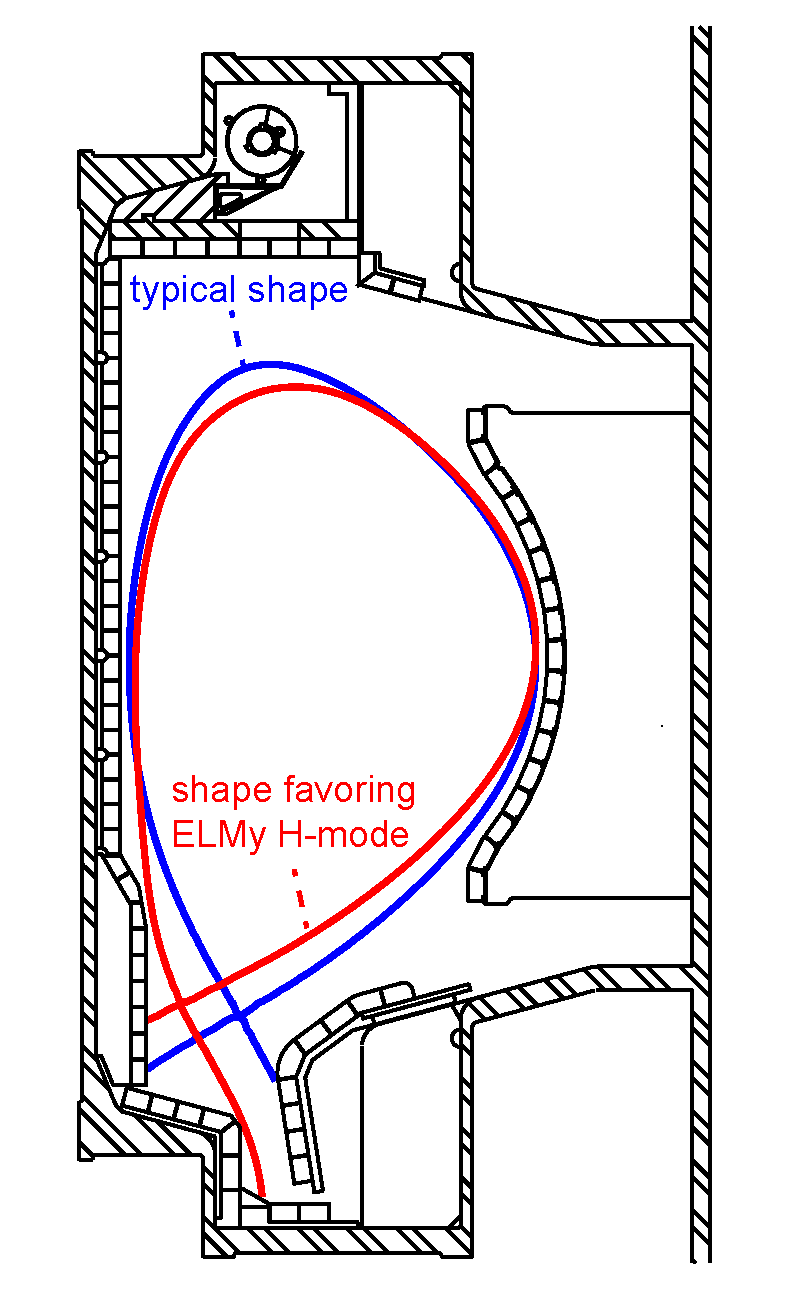
\includegraphics[width=90mm]{graphics/ELMy/shaping.pdf}}
\end{figure}

High-confinement operation on Alcator C-Mod differs is unique among major tokamak experiments in that typical H-modes do not exhibit the large Type-I ELMs customarily seen on other devices \cite{Greenwald2007}.  Instead, ELM-free H-modes tend to form at lower collisionalities heating power levels, with high-density, high-power operation tending towards the continuously-regulated EDA H-mode rather than exhibiting discrete ELMs (see \cref{sec:hcr_elmfree,subsec:hcr_eda}).  However, by operating in a modified shape (see \cref{fig:elmy_shaping}) with low elongation, $\kappa \sim 1.4-1.5$, and upper triangularity ($\delta_u \sim 0.15$) paired with high lower triangularity ($\delta_l > 0.75$) and a strike point on the divertor floor, regular ELMy H-mode operation is attainable.  This comparatively weak shaping, developed in similarity experiments with the JFT-2M tokamak \cite{Hughes2011,Terry2007a}, reduces the necessary pressure gradient and bootstrap current to reach the ideal peeling-ballooning MHD stability 
boundary (described in \cref{sec:mod_pb}), triggering the ELM.  In this shape, new experiments on C-Mod \cite{Walk2012} attained ELMy H-modes across a broad range in current ($400-1100 \;\si{\kilo\ampere}$) and field ($3.5-8 \;\si{\tesla}$) with high-resolution pedestal data.

\begin{figure}[t]
 \pushtooutside
 \ffigbox[\FBwidth]{
\includegraphics[width=150mm]{graphics/ELMy/time_window.pdf}}{\caption[Example time window for ELMy H-mode study, showing TS timebase.]{Example ELMy H-mode window (highlighted).  Phases for study are selected for steady density ($\overline{n}_e$ shown in the top trace), temperature (ECE $T_e$ signals shown for the core and pedestal), and ELM cycles ($D_\alpha$ signal shown).  The same modeling window is shown zoomed-in at the right.  Note the strong perturbation to the edge temperature due to the sawtooth crash.  Thomson scattering frames are indicated by the black ticks on the axes -- the ELM cycle is at a comparable frequency, $\sim \SI{60}{\hertz}$, to the TS system frame rate.  This presents a difficulty for selecting data masked to the ``peak'' of the ELM cycle, necessitating long, steady ELMing phases for study.}\label{fig:elmy_timewindow}}
\end{figure}

\begin{figure}
 \pushtooutside
 \ffigbox[\FBwidth]{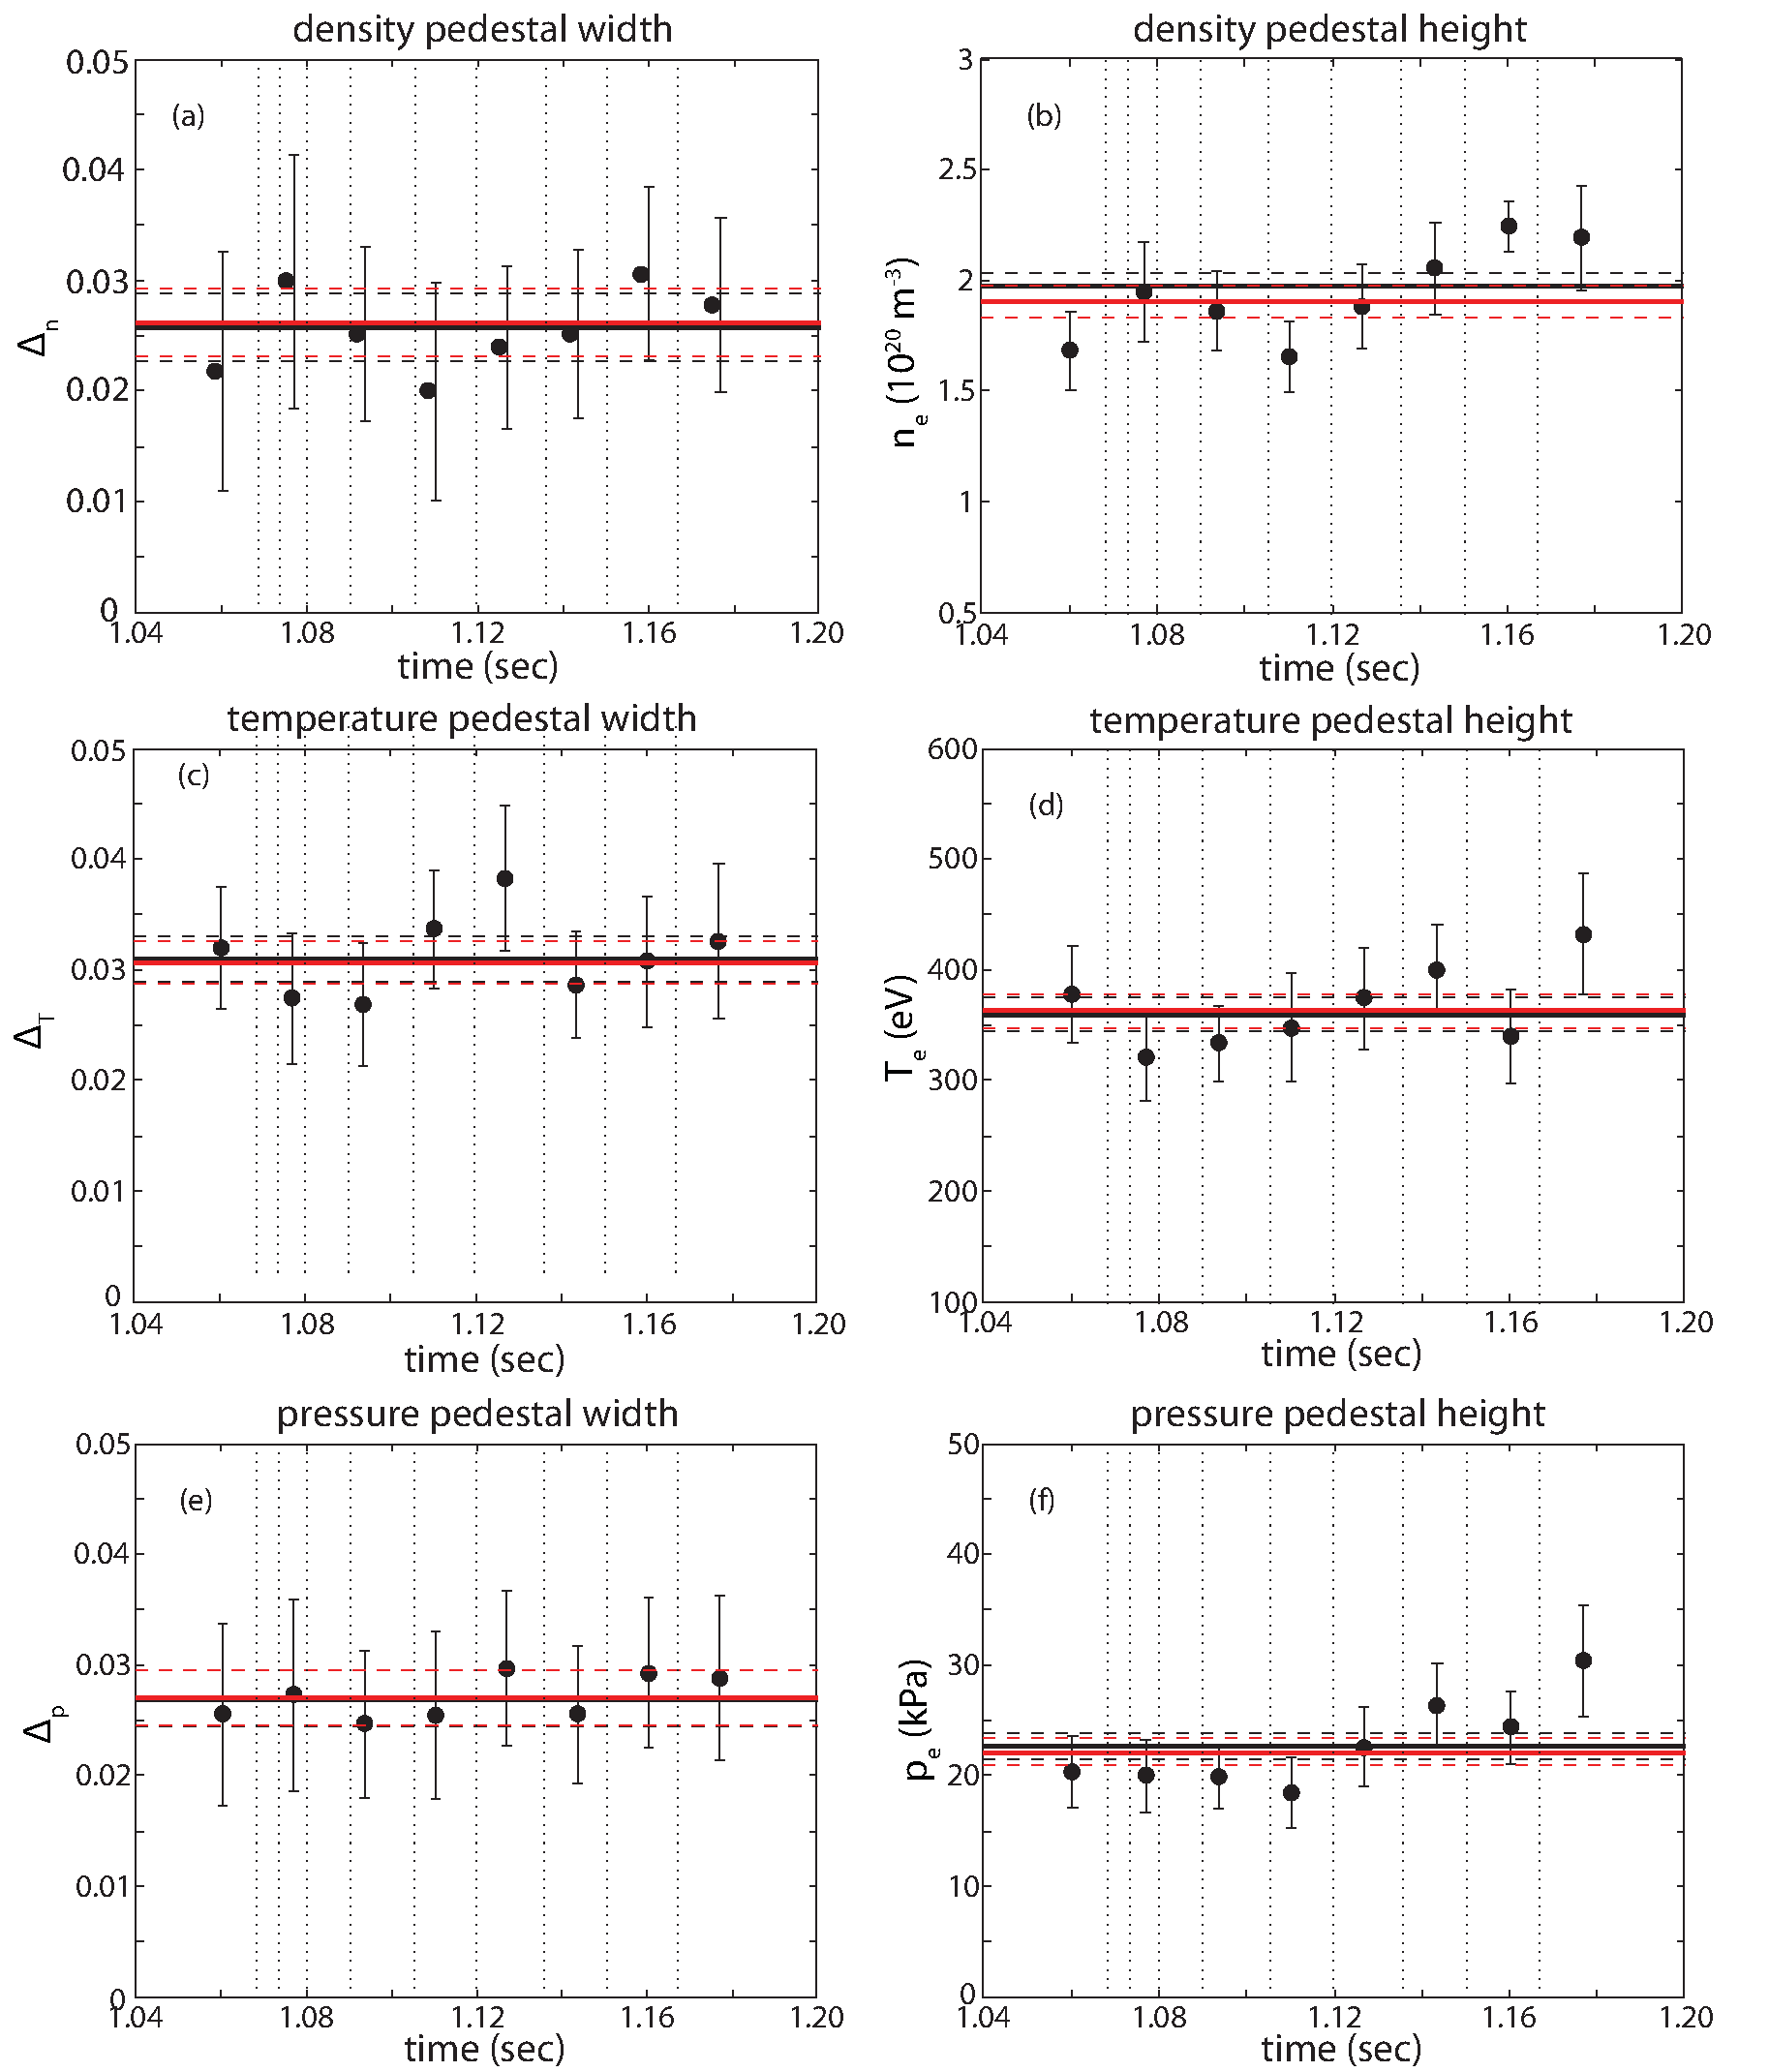
\includegraphics[width=150mm]{graphics/ELMy/ensemble.pdf}}{\caption[Comparison of pedestal fits for individual frames versus ensemble average.]{Comparison of fits for the $n_e$, $T_e$, and $p_e$ pedestal width and height from Thomson scattering.  Individual frames of data are shown as black points, with their average shown by the black line (errorbars indicated by the dashes).  The ensemble-averaged fit is shown in red.  The ensemble fit captures the average behavior in a steady ELMing phase well, while suppressing the random scatter found in indivual frames of TS data.  For comparison, ELM crash times in the window are indicated by vertical dashed lines.}\label{fig:elmy_ensemble}}
\end{figure}


Pedestal profiles are taken with the edge Thomson scattering system, detailed in \cref{subsec:app_ts_cmod}.  The pedestal data is taken over steady ELMing phases to minimize the effects of random scatter in the data -- an example of such a window, with line-averaged density $\overline{n}_e$, core and edge $T_e$, and divertor $D_\alpha$ signal (indicative of the ELM crash), is shown in \cref{fig:elmy_timewindow}, with a comparison of the individual-frame fits to the ensemble shown in \cref{fig:elmy_ensemble}.  Strictly, models of the pedestal structure in ELMy H-mode predict the pedestal immediately preceding the ELM crash, when the pedestal is most unstable to the ELM trigger.  However, ELMs on C-Mod typically cycle at $60-100 \;\si{\hertz}$, comparable to the repetition rate of the Thomson scattering system (as shown in \cref{fig:elmy_timewindow,fig:elmy_ensemble}).  This presents difficulties in resolving the pedestal with multiple frames per ELM and binning the data to the peaks of the ELM cycle.  In most 
cases, pedestals are prepared in a single ``ensemble average'' utilizing all TS data in the window; in certain cases, a statistical set is also constructed using the last 20\% of the ELM cycle as is typical for other machines.  The results from this correction are discussed in \cref{sec:elmy_sync}.

\begin{figure}
 \pushtooutside
 \fcapside[65mm]{\caption[Example pedestal illustrating the $mtanh$ fitting function.]{Example pedestal illustrating the $mtanh$ function used for pedestal fitting (\cref{eq:mtanh}), defining the parameters: height $h$, baseline $b$, midpoint $x_0$, half-width $\delta$/full width $\Delta$.  The inboard slope is characterized by the parameter $\alpha$.}\label{fig:mtanh}}{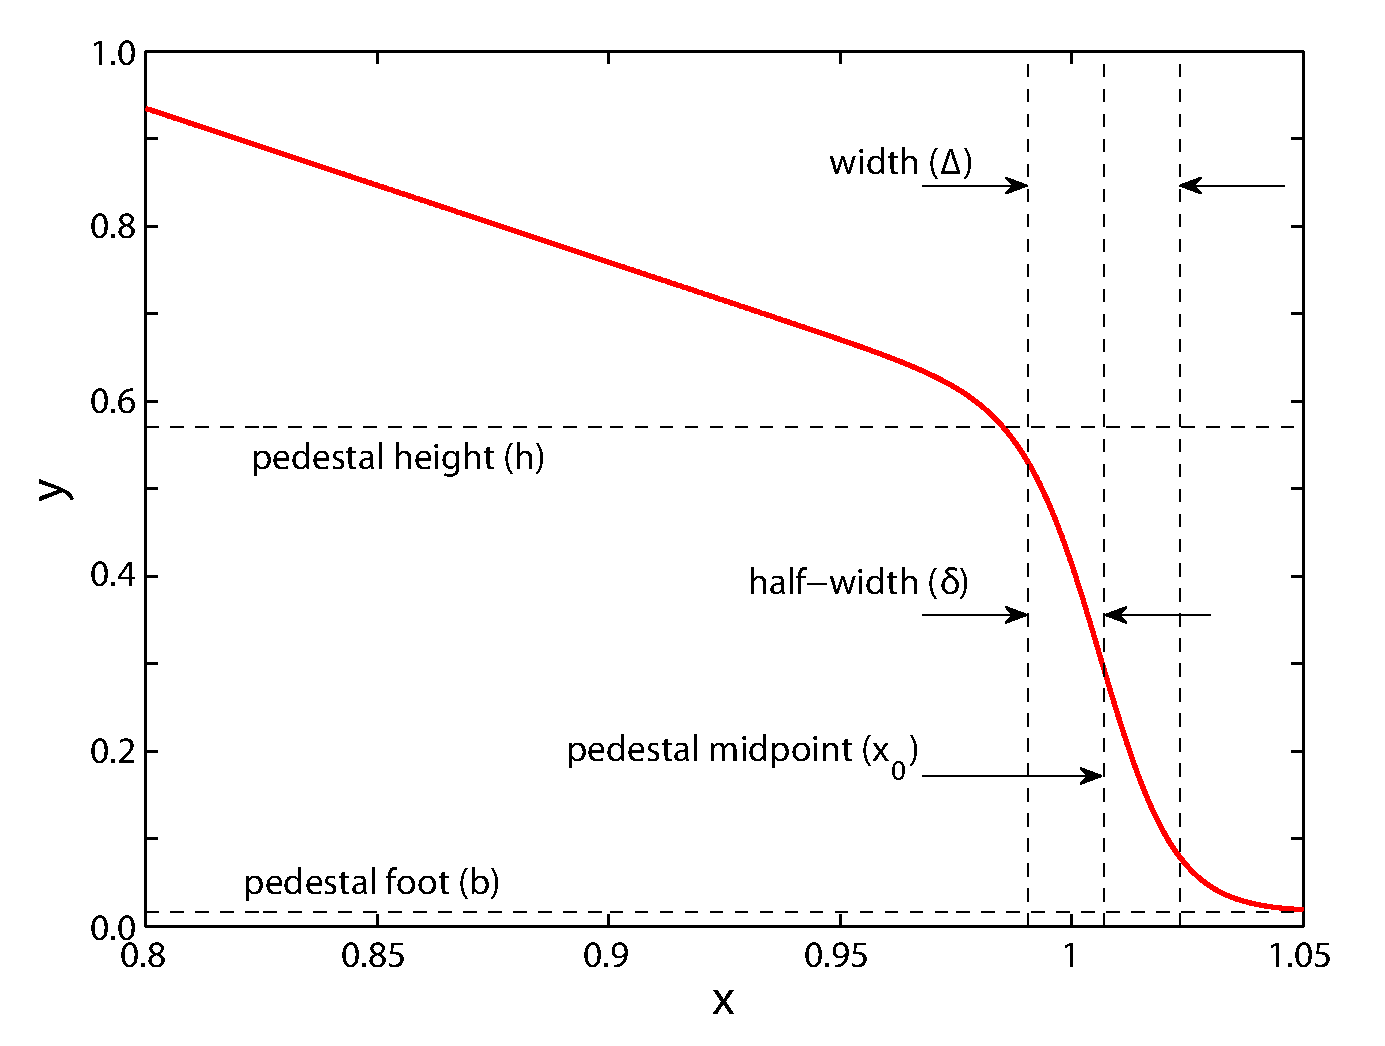
\includegraphics[width=100mm]{graphics/ELMy/mtanh.pdf}}
\end{figure}

The electron density, temperature, and pressure profiles are fitted using a modified hyperbolic-tangent fit developed in \cite{Groebner2001}.  In a general $x,y$ space, the fitting function is expressed by

\begin{equation}\label{eq:mtanh}
 \begin{aligned}
  z &= \frac{x_0 - x}{\delta}\\
  mtanh(\alpha,z) &= \frac{(1 + \alpha z) e^z - e^{-z}}{e^z + e^{-z}}\\
  y &= \frac{h+b}{2} + \frac{h-b}{2} mtanh(\alpha,z)
 \end{aligned}
\end{equation}

\noindent where $x_0$ is the pedestal midpoint, $h$ and $b$ are the height and baseline, and $\delta$ is the half-width (we use $\Delta = 2\delta$ as the ``pedestal width'').  The inboard slope is encoded by the parameter $\alpha$, with the multiplicative factor $1 + \alpha z$ providing an approximately linear profile inboard from the steep-gradient region.  This definition provides a smooth, continuous definition for the pedestal gradient throughout the profile, with the peak gradient found analytically at $x_0$.  Recent H-mode studies use the fitting parameter $h$ as the figure-of-merit for the pedestal height; however, it is also common to express the pedestal height in terms of the evaluated value of the fit at the 95\% poloidal flux surface.  For the purposes of this document we denote the height taken from the fitting parameter $h$ by the subscript $ped$, and values taken at the 95\% flux surface by the subscript $95$. 

Due to the ready availability of high-resolution electron density and temperature diagnostics, for the purposes of this section we assume equal ion and electron pressures, $p = 2n_e T_e$ (a viable approximation on C-Mod due to the relatively low impurity content found in ELMy H-modes, $Z_{eff} \sim 2$, and rapid ion-electron equilibration in H-mode pedestals on C-Mod \cite{McDermott2009a}).  All profiles are prepared using normalized poloidal flux for the abscissa, facilitating comparison to results from other machines and to the EPED model.  For the purposes of the EPED model we also prepare an averaged width, defined by

\begin{equation}\label{eq:wid_eped}
  \delta_\psi = \frac{\delta_{n_e} + \delta_{T_e}}{2}\qquad
  \Delta_\psi = 2\delta_\psi
\end{equation}

\noindent a practice necessitated by cases in which the density and temperature profile measurements are generated by distinct diagnostics (rather than taking both from the Thomson scattering system, as is customary on C-Mod).  As the density and temperature widths are quite close (although the density pedestal is, on average, slightly wider, as shown in \cref{fig:elmy_deltan_deltaT}, with an average ratio of $\Delta_{T_e}/\Delta_{n_e} = 1.051$), the difference between $\Delta_\psi$ and the directly-measured $\Delta_{p_e}$ is minimal -- as shown in \cref{fig:elmy_deltap_deltapsi}, the two widths are well-correlated, with $\Delta_\psi$ systematically slightly wider.\nicesectionending

\begin{figure}
 \pushtooutside
 \begin{floatrow}
  \ffigbox[\FBwidth]{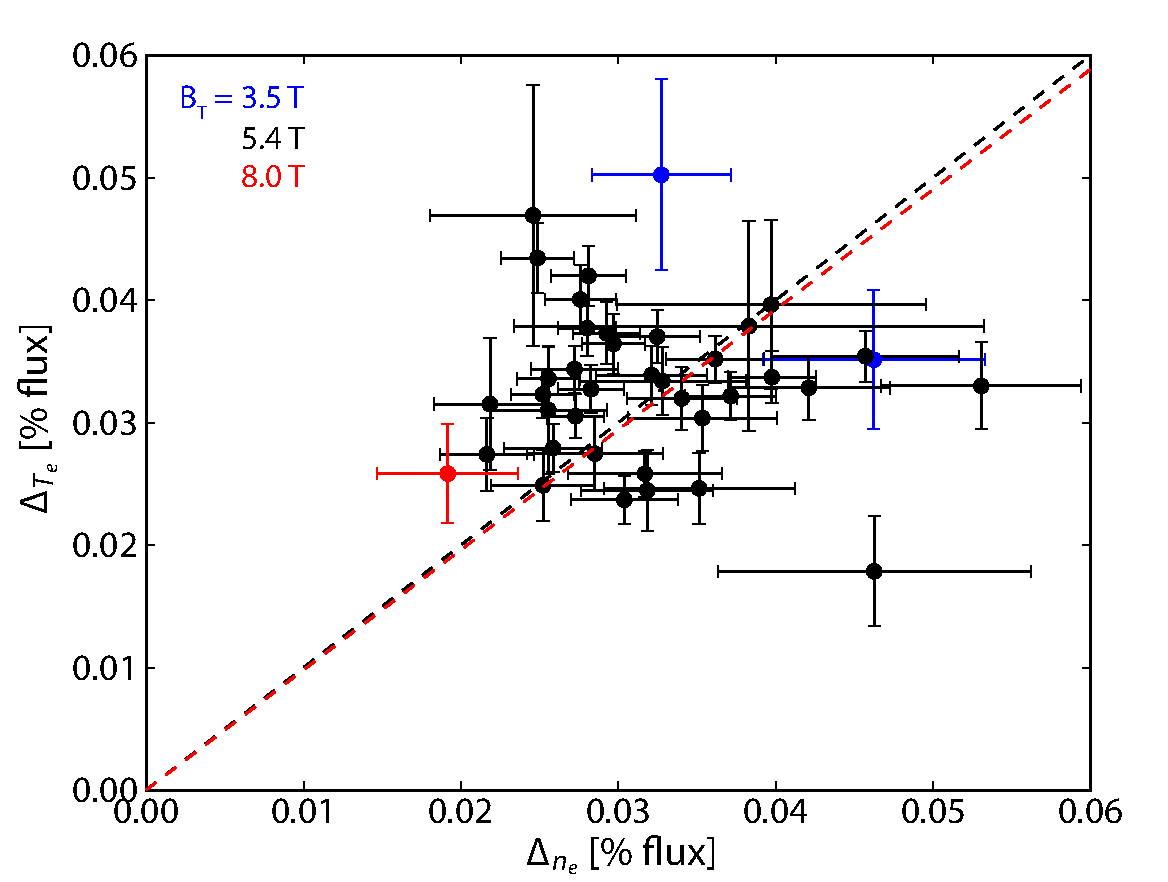
\includegraphics[width=75mm]{graphics/ELMy/deltan_deltaT.pdf}}{\caption[Comparison of measured $n_e$ and $T_e$ pedestal widths.]{Comparison of the measured pedestal widths for the $n_e$ and $T_e$ pedestals, differentiated for the low-, standard-, and high-field H-mode cases.  Pedestal widths are similar for density and temperature, although on average the density pedestal is slightly wider.  The error-weighted centroid of the dataset is shown by the star.}\label{fig:elmy_deltan_deltaT}}
  \ffigbox[\FBwidth]{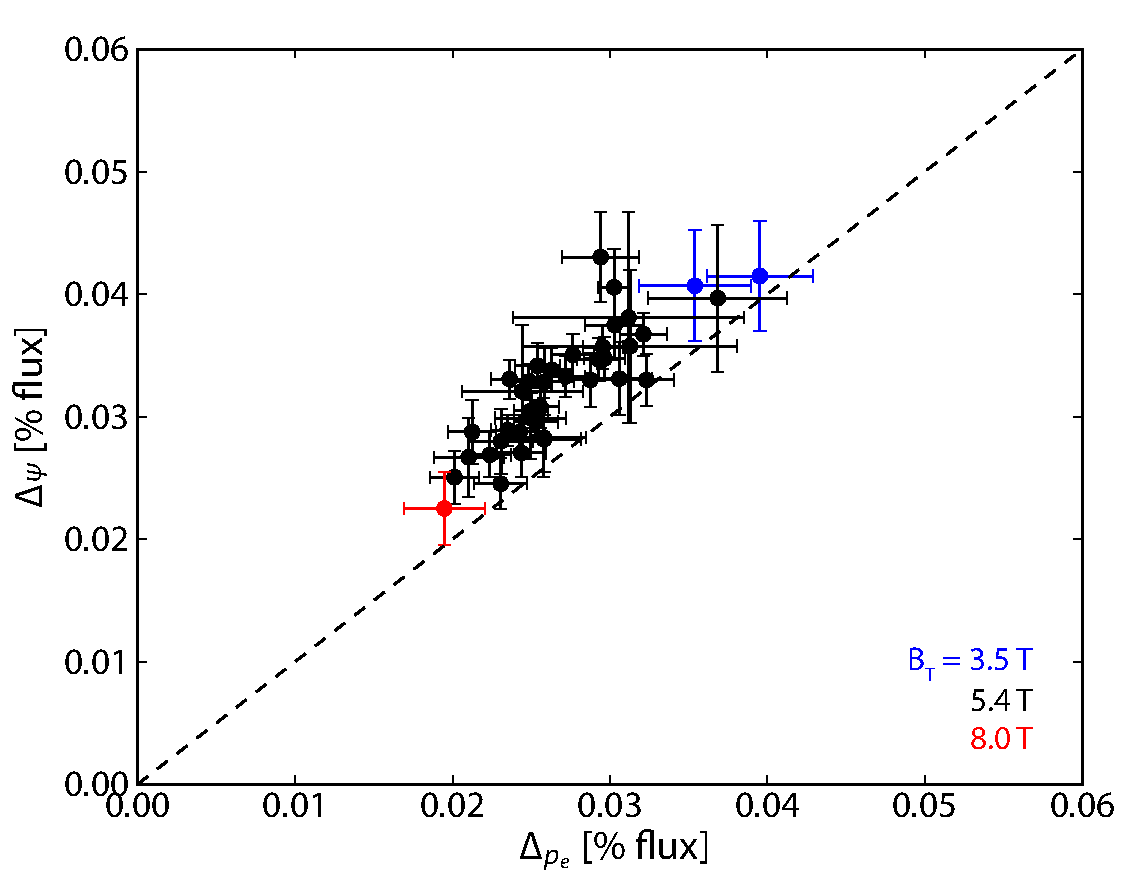
\includegraphics[width=75mm]{graphics/ELMy/deltap_deltapsi.pdf}}{\caption[Comparison of directly measured pressure pedestal width versus EPED pedestal width.]{Comparison of the directly-measured pressure pedestal width and the EPED width $\Delta_\psi$ defined as the average of $\Delta_{n_e}$ and $\Delta_{T_e}$.  The widths trend quite closely to one another, although $\Delta_\psi$ is systematically somewhat wider.}\label{fig:elmy_deltap_deltapsi}}
 \end{floatrow}
\end{figure}

\section{ELM Cycle Synchronization}\label{sec:elmy_sync}

The common practice for modeling the ELMy H-mode pedestal is to take profile data immediately preceding the ELM crash (commonly, data from the last 20\% of the ELM cycle), as this most closely corresponds to the pedestal profile at the stability limit associated with the ELM trigger.  However, as the ELM cycle in H-mode on C-Mod is typically at a comparable repetition rate to the Thomson Scattering system ($\SI{60}{\hertz}$), this practice is only possible on a subset of discharges, with sufficiently long, steady H-mode phases, such that a sufficient number of frames in the desired time wondow can be found.

\begin{figure}[h]
 \pushtooutside
 \fcapside[60mm]{\caption[Comparison of pressure pedestal height between ensemble-averaged and ELM-synced profiles.]{Comparison of the pressure pedestal height $p_{ped}$ between the ensemble-averaged and ELM-synchronized profiles.  On average, ELM synchronization results in a 10.8\% increase in measured pedestal pressure, consistent with ELM losses observed on other machines.  At lower pressures, ELMs are typically small enough that the perturbation is minimal; however, the distinction becomes important for the highest-pressure ELMy H-modes on C-Mod.}\label{fig:elmy_pped_ens_elmsync}}{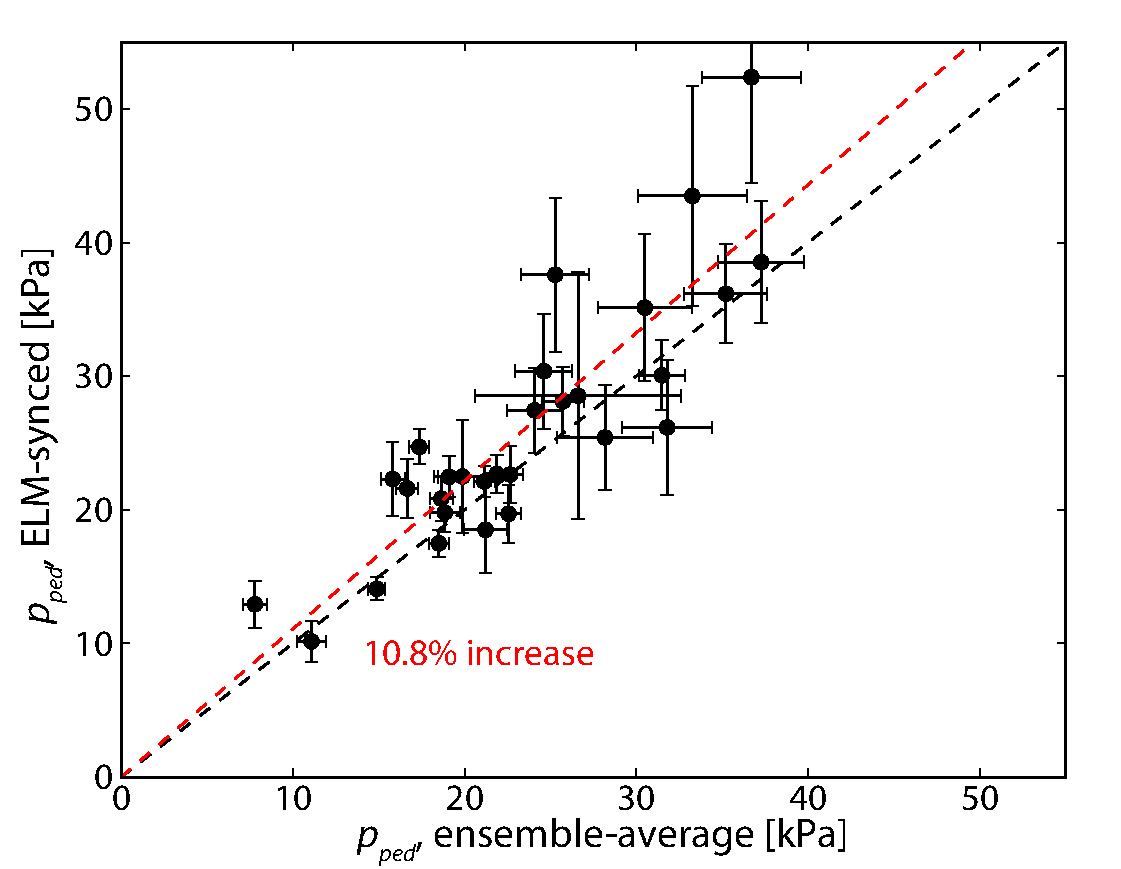
\includegraphics[width=100mm]{graphics/ELMy/pped_ensemble_elmsync.pdf}}
\end{figure}

\begin{figure}[h]
 \pushtooutside
 \fcapside[60mm]{\caption[Comparison of pressure at the 95\% flux surface between ensemble-averaged and ELM-synced profiles.]{Comparison of the pressure at the 95\% flux surface, $p_{95}$, between the ensemble-averaged and ELM-synchronized profiles.  On average, ELM synchronization results in a 7.6\% increase in the measured pressure.  This is consistent with the ELM perturbation to the pedestal being largely restricted to the pedestal just within the steep-gradient region, with decreasing perturbation further into the plasma from the pedestal.}\label{fig:elmy_p95_ens_elmsync}}{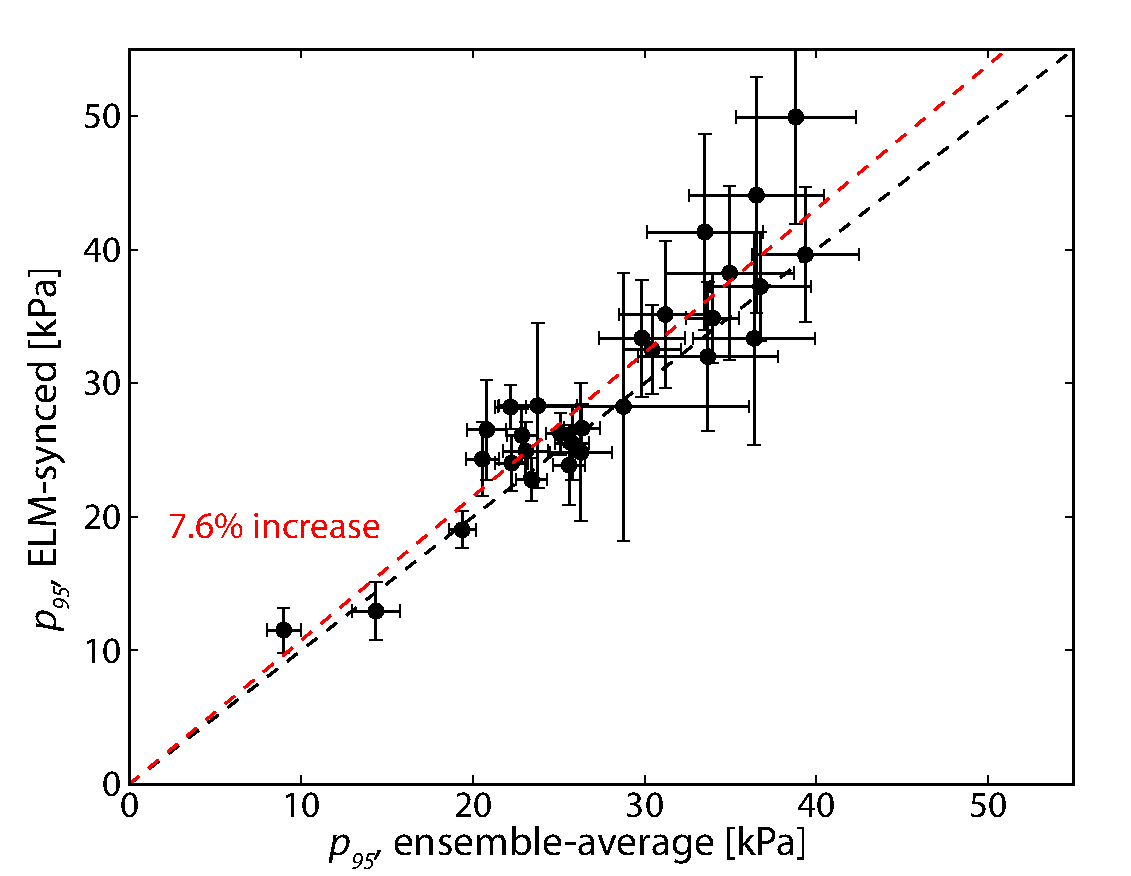
\includegraphics[width=100mm]{graphics/ELMy/p95_ensemble_elmsync.pdf}}
\end{figure}

A comparison between the ensemble-averaged and ELM-synchronized pressure pedestals (pedestal height $p_{ped}$ and the pressure at the 95\% flux surface $p_{95}$) are shown in \cref{fig:elmy_pped_ens_elmsync,fig:elmy_p95_ens_elmsync}.  ELM synchronization finds an average 10.8\% increase in the measured pressure $p_{ped}$, with a slightly lesser increase of 7.6\% in $p_{95}$.  This is consistent with the perturbation to the pressure pedestal by the ELM observed on other machines \cite{Urano2003,Loarte2003}.  The weaker perturbation due to the ELM crash observed at the 95\% flux surface is also consistent with previous ELM observations -- the ELM crash typically alters the pressure profile only in a region just inside the steep-gradient region, with minimal perturbation to profiles in the plasma interior.\nicesectionending

\section{EPED Model Predictions}\label{sec:elmy_eped}

The EPED model, described in \cref{sec:mod_eped}, combines pedestal limits based on coupled peeling-ballooning MHD instabilities \cite{Snyder2004,Wilson2002,Wilson2006} and kinetic-ballooning mode turbulence \cite{Snyder2001}.  These models set two distinct constraints on the pedestal width and height, with peeling-ballooning MHD predicting $p_{ped} \sim \Delta^{3/4}$ and kinetic-ballooning turbulence predicting $p_{ped} \sim \Delta^2$\gnote{reference figure in chapter 3, probably}.  The unique intersection of these two constraints provides a predictive value for the pedestal width and height.  The most recent version of the model, EPED1.63, utilizes gyrokinetic calculations to more accurately constrain the KBM limit, and includes a modified term accounting for the strong diamagnetic stabilization of high-$n$ modes in the pedestal on C-Mod.  A comparison between the observed and predicted pedestal parameters is presented here.

\subsection{Pedestal Height}\label{subsec:elmy_eped_height}

A comparison between the pressure pedestal height predicted by EPED1.63 and the observed height is shown in \cref{fig:elmy_pped_EPED_meas}.  While most measured pedestals lie within the $\pm 20\%$ expected error in the EPED prediction (indicated by the grey band in \cref{fig:elmy_pped_EPED_meas}), the EPED model systematically over-predicts the pedestal pressure, corresponding on average ratio of measured to predicted pedestal heights of $0.835 \pm 0.036$, indicated by the red dashed line.

\begin{figure}[h]
 \pushtooutside
 \fcapside[60mm]{\caption[Pressure pedestal height predicted by EPED versus measured (ensemble-averaged) height.]{Pressure pedestal height predicted by EPED1.63 versus the measured (ensemble-averaged) pedestal height, color-coded by magnetic field set.  The grey band indicates perfect agreement, $\pm 20\%$ typical prediction accuracy for EPED.  The EPED model systematically over-predicts the pedestal pressure, with an average match of $0.835 \pm 0.036$ (indicated by the red line).}\label{fig:elmy_pped_EPED_meas}}{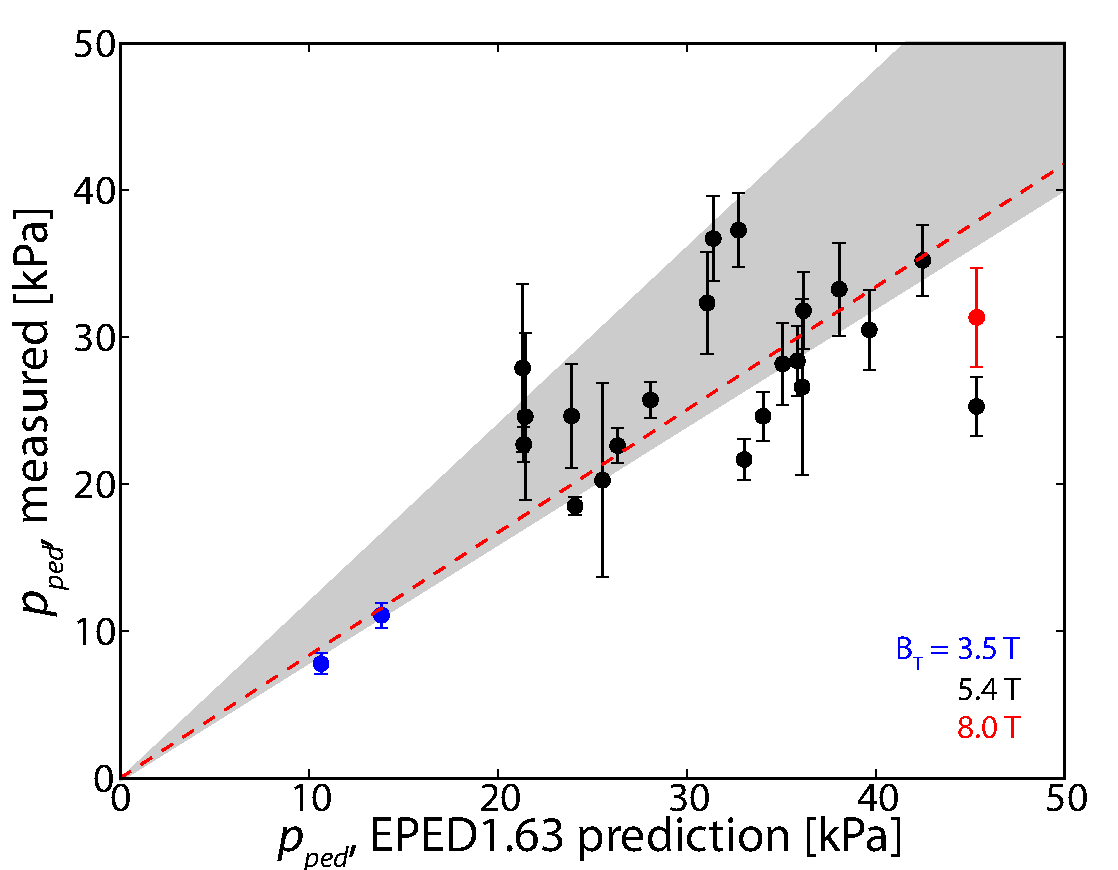
\includegraphics[width=100mm]{graphics/ELMy/pped_EPED_meas.pdf}}
\end{figure}

The discrepancy between the predicted and measured pedestal heights may be attributed (at least in part) to the use of pedestal measurements averaged across the entire ELM cycle (``ensemble-averaged'').  As discussed in \cref{sec:elmy_sync}, models of the pedestal structure (including EPED) most closely correspond to the pedestal structure immediately preceding the ELM crash, where the pedestal is most unstable to the ELM trigger.  A subset of ELMy H-modes are prepared with ELM-synchronized data, shown in \cref{fig:elmy_pped_EPED_sync} with the corresponding ensemble-averaged points for comparison.  The prediction accuracy is substantially improved, with an average ratio of measured to predicted pedestal heights of $0.934 \pm 0.066$, well within the anticipated $\pm 20\%$ accuracy of the EPED prediction.  As expected, the modification to the measured pedestal pressure by ELM synchronization is minimal at lower pedestal pressures, but becomes substantial at higher pedestal pressures ($> \SI{35}{\kilo\pascal}$)
 as ELM losses increase proportionally with the pedestal stored energy.

The EPED model still systematically slightly over-predicts the pedestal pressure, however -- this is potentially due to the strong sensitivity of the stability calculation to diamagnetic effects, which tend to stabilize higher-$n$ ballooning modes.  As diamagnetic effects are substantial in the relatively collisional pedestal found in H-modes on C-Mod, a careful accounting of these effects is necessary for accurate prediction -- use of a slightly weaker diamagnetic stabilization model brings the prediction into generally better agreement with C-Mod data.

\begin{figure}[t]
 \pushtooutside
 \fcapside[60mm]{\caption[Pressure pedestal height predicted by EPED versus measured ELM-synced pedestal height.]{Pressure pedestal height predicted by EPED1.63 versus measured, ELM-synchronized pedestal height (red, with corresponding ensemble-average points shown in black).  The grey band indicates perfect agreement, $\pm 20\%$ typical prediction accuracy for EPED.  ELM synchronization brings the measured pedestal height into better agreement with EPED predictions, with a correspondence of $0.934 \pm 0.066$ (indicated by the red dash).}\label{fig:elmy_pped_EPED_sync}}{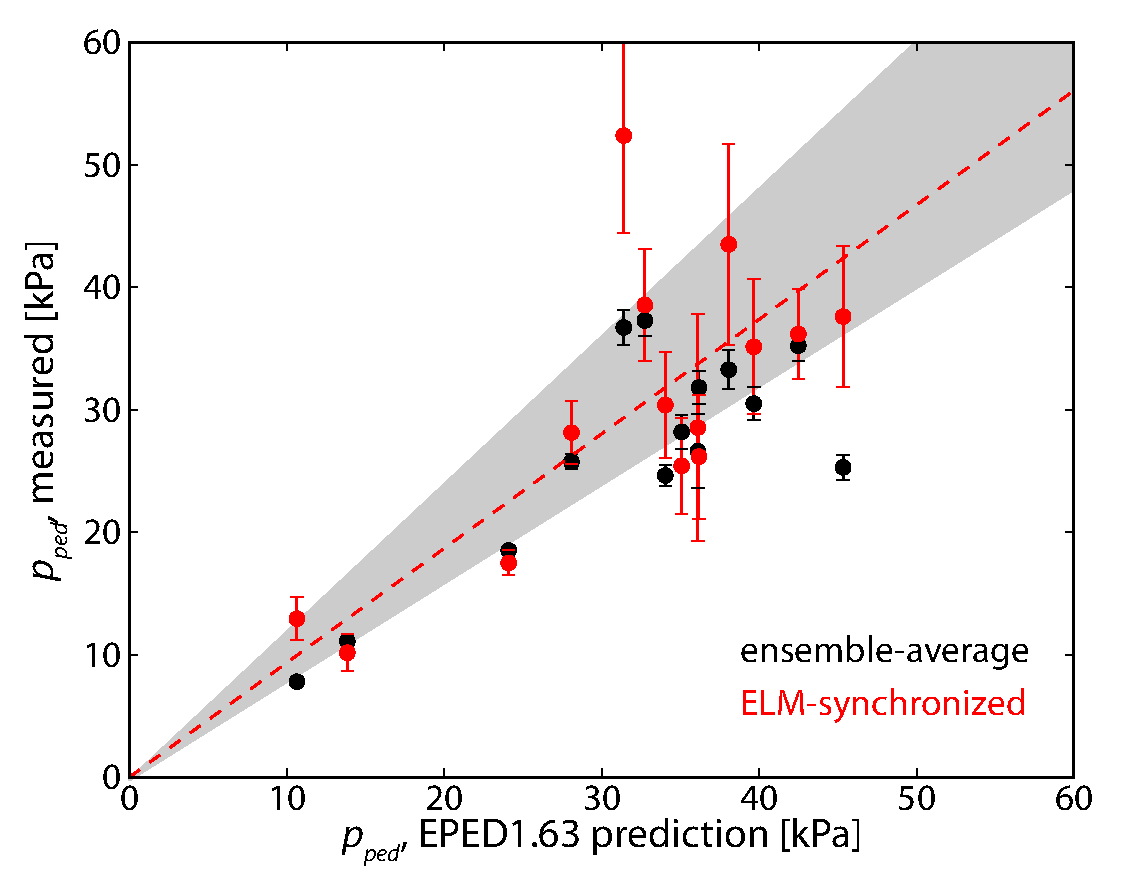
\includegraphics[width=100mm]{graphics/ELMy/pped_EPED_elmsync.pdf}}
\end{figure}

\subsection{Pedestal Width}\label{subsec:elmy_eped_width}

While historically a number of models for the pedestal width (see \cref{sec:mod_early}) have been examined, the most uniformly successful has been an expected scaling of pedestal width with poloidal beta at the pedestal top ($\beta_{p,ped}$), observed on several machines \cite{Groebner2013}, and shown to follow from a critical-gradient limit in the edge pressure profile established by kinetic-ballooning mode (KBM) turbulence.  Including magnetic shear stabilization, this takes the form $\Delta = c \beta_{p,ped}^{1/2}$, where $c$ is, strictly, a weakly-varying function of a number of plasma parameters \cite{Snyder2009}.  This constraint on the pedestal width and height is utilized in the EPED model, coupled with peeling-ballooning MHD stability limits to set a unique constraint on the pedestal structure at the ELM crash.

An evaluation of this scaling with ensemble-averaged data is shown in \cref{fig:elmy_betap_deltapsi_all}, with a fitted scale factor of $\langle c \rangle = 0.0857 \pm 0.0024$, consistent with previously-observed scalings.  The earliest versions of the EPED model used this simple constraint as the second condition on the pedestal width and height, using an experimentally-determined fixed scale factor.  The newest version of the model self-consistently calculates the scale factor from gyrokinetic considerations of the KBM turbulence; however, the results is quantitatively similar.  A comparison of the experimental versus the EPED1.63-predicted pedestals in $\Delta_\psi - \beta_{p,ped}$ space is shown in \cref{fig:elmy_betap_deltapsi_EPED}.

\begin{figure}[ht]
 \pushtooutside
 \fcapside[60mm]{\caption[Ensemble-averaged $\Delta_\psi$ versus $\beta_{p,ped}$.]{Ensemble-averaged EPED width $\Delta_\psi$ (\cref{eq:wid_eped}) versus $\beta_{p,ped}$, color-coded by field set.  The expected scaling from the KBM limit, $\Delta_\psi = c \beta_{p,ped}^{1/2}$, is shown with a scale factor of $0.0857$, consistent with observations in previous experiments.}\label{fig:elmy_betap_deltapsi_all}}{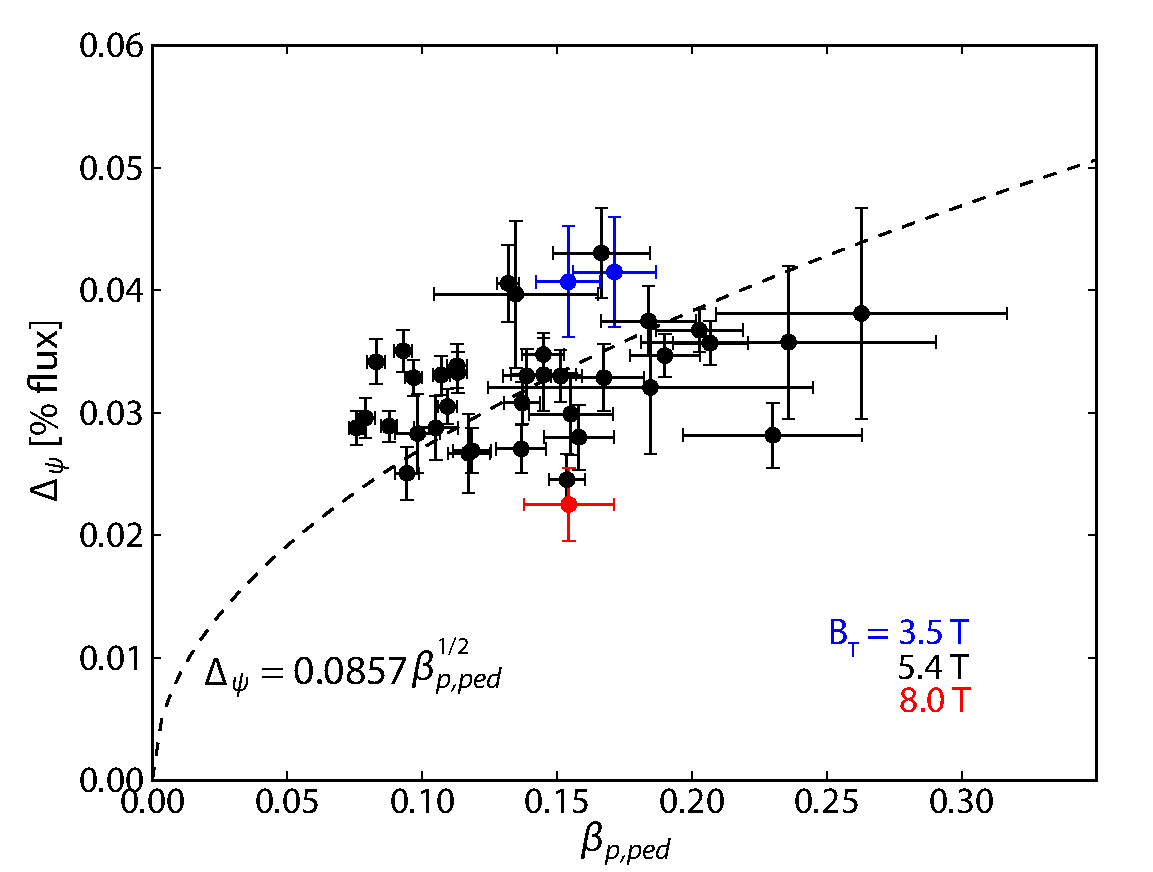
\includegraphics[width=100mm]{graphics/ELMy/betap_deltapsi_all.pdf}}
\end{figure}

\begin{figure}[ht]
 \pushtooutside
 \fcapside[60mm]{\caption[Comparison of EPED-predicted pedestal width and height with corresponding experimental points.]{Comparison of EPED1.63-predicted pedestal width $\Delta_\psi$ and height $\beta_{p,ped}$ with the corresponding ensemble-averaged experimental points, with the KBM scaling $\Delta_\psi = c \beta_{p,ped}^{1/2}$.  Though the EPED predictions were calculated with a self-consistent treatment of the scale factor $c$ as a weakly-varying function of plasma parameters, the result is quantitatively similar to the simple fixed scale factor.}\label{fig:elmy_betap_deltapsi_EPED}}{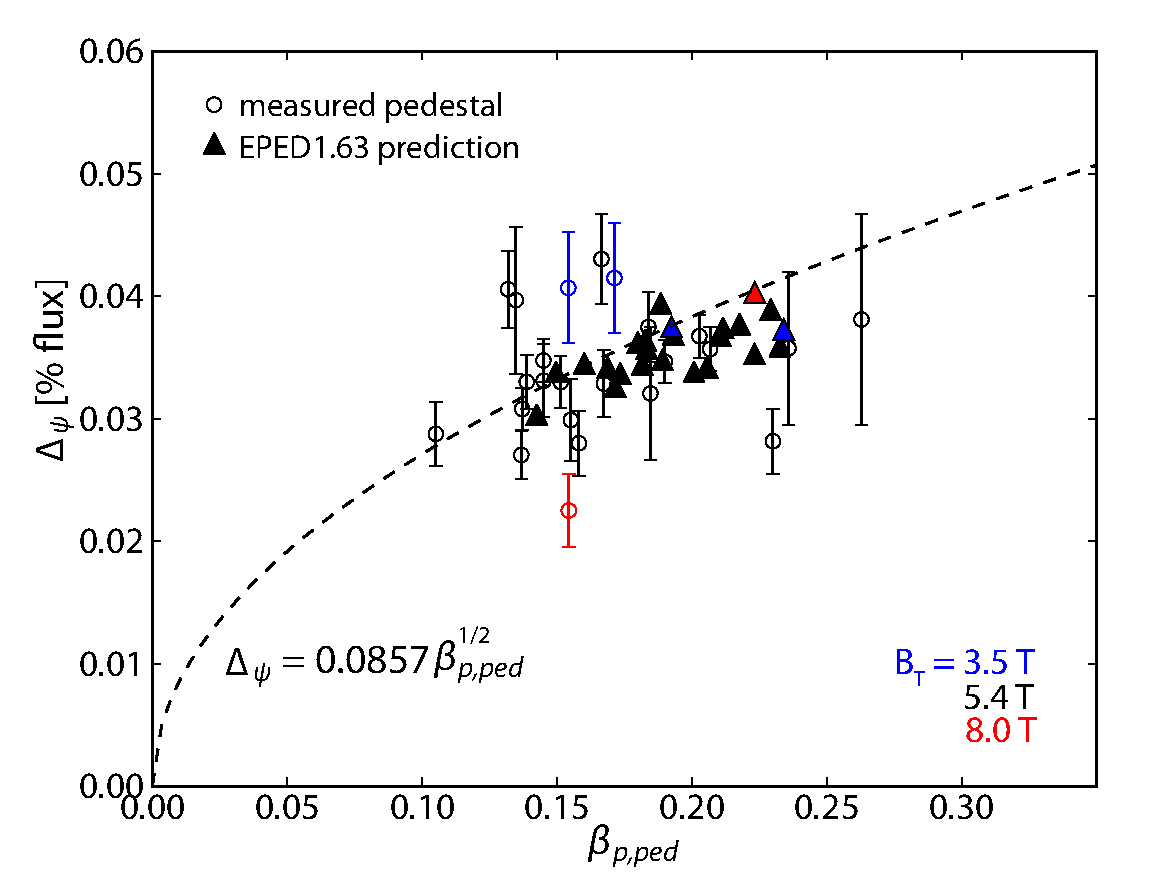
\includegraphics[width=100mm]{graphics/ELMy/betap_deltapsi_EPED.pdf}}
\end{figure}

Application of the ELM synchronization technique does not significantly alter this result, although the pedestal pressure (\ie $\beta_{p,ped}$) is significantly increased in the last 20\% of the ELM cycle.  Recent research in the inter-ELM development of the pedestal \cite{Diallo2014} has shown that the KBM saturates early in the ELM cycle, limiting the pedestal gradient; the pedestal width and height then both increase until the peeling-ballooning MHD boundary is also reached, triggering the ELM.  Consistent with this, ELM-synchronized pedestals exhibit wider, taller pedestals on average, with a similar constraint imposed by the KBM compared to the ensemble-averaged result\gnote{check reasoning!}.  A comparison of the ensemble-averaged and ELM-synced pedestals in $\Delta_\psi - \beta_{p,ped}$ space is shown in \cref{fig:elmy_betap_deltapsi_elmsync}, with the ELM-synced pedestals fitted to a scale factor $\langle c \rangle = 0.0896 \pm 0.0034$.  The data may be clarified significantly by taking an error-
weighted average within fixed bins in $\beta_{p,ped}$ as well, shown in \cref{fig:elmy_betap_deltapsi_betabin}, which tends to reduce the influence of strongly-outlying points on the fit.  Again, the fit is quantitatively very similar -- the data fit well to $\Delta_\psi = c \beta_{p,ped}^{1/2}$ with $\langle c \rangle = 0.0851 \pm 0.003$.  Alternately, we may use a more general power-law fit $\Delta_\psi = c_1 \beta_{p,ped}^{c_2}$, with which we find $\langle c_1 \rangle = 0.0824 \pm 0.015$ and $\langle c_2 \rangle = 0.49 \pm 0.11$, closely reproducing the $\beta_{p,ped}^{1/2}$ model.  The fitting results are quite consistent across these methods, demonstrating the robustness of the KBM model for the pedestal width and its insensitivity to the details of data preparation.

\begin{figure}[t]
 \pushtooutside
 \fcapside[60mm]{\caption[Comparison of ensemble-averaged and ELM-synced pedestal width and height, compared to the KBM constraint.]{Comparison of ensemble-averaged (black) and ELM-synchronized (Red) pedestal width and height, compared to the KBM constraint.  The $\Delta_\psi = 0.0857 \beta_{p,ped}^{1/2}$ scaling found in the ensemble-averaged case is shown in black, while the minor modification of $\Delta_\psi = 0.0896 \beta_{p,ped}^{1/2}$ for the ELM-synced cases is shown in red.}\label{fig:elmy_betap_deltapsi_elmsync}}{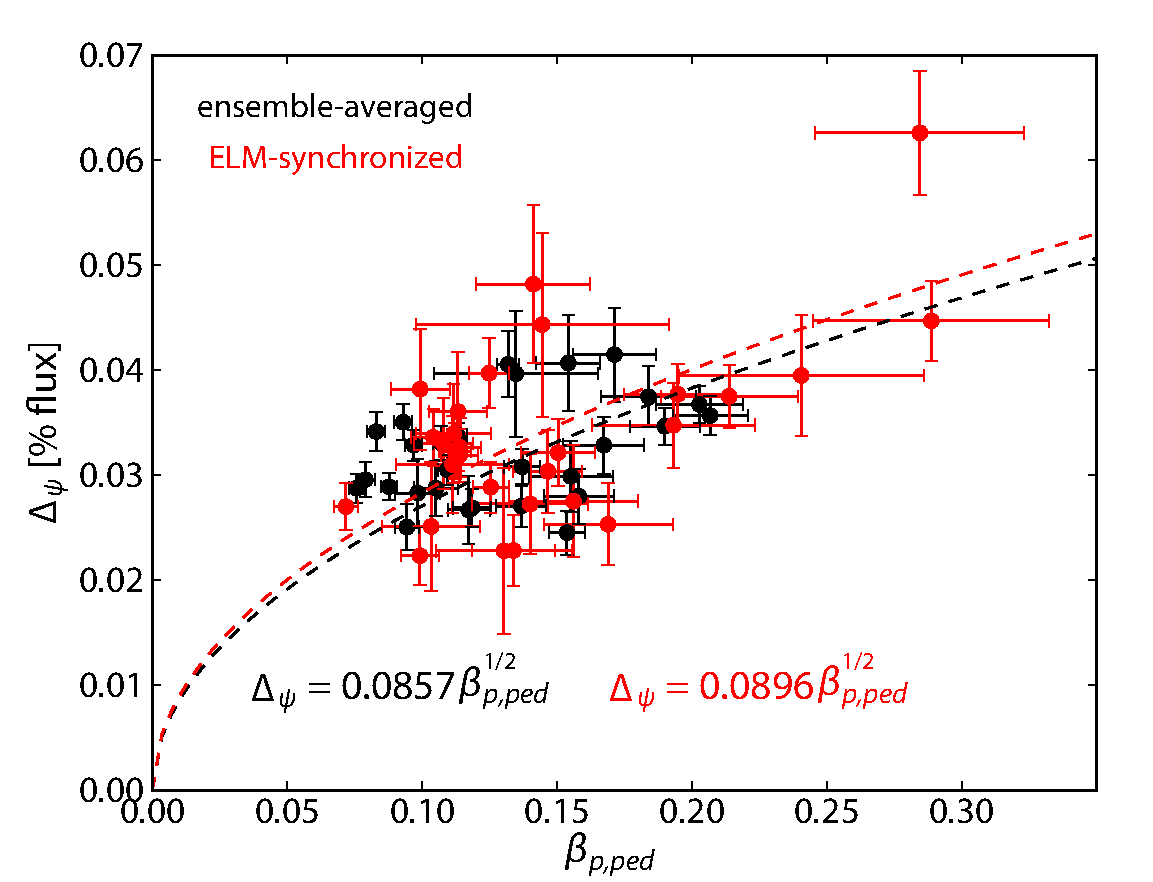
\includegraphics[width=100mm]{graphics/ELMy/betap_deltapsi_elmsync.pdf}}
\end{figure}

\begin{figure}[ht]
 \pushtooutside
 \fcapside[60mm]{\caption[ELM-synced pedestals with data binned by $\beta_{p,ped}$, fitted to $\Delta_\psi \sim \beta_{p,ped}^{1/2}$.]{ELM-synchronized pedestals, with data binned by $\beta_{p,ped}$ for clarity.  The data are fitted by $\Delta_\psi = (0.0851 \pm 0.003) \beta_{p,ped}^{1/2}$ (black), or by $\Delta_\psi = (0.0824 \pm 0.015) \beta_{p,ped}^{0.49 \pm 0.11}$ using a more general power law.}\label{fig:elmy_betap_deltapsi_betabin}}{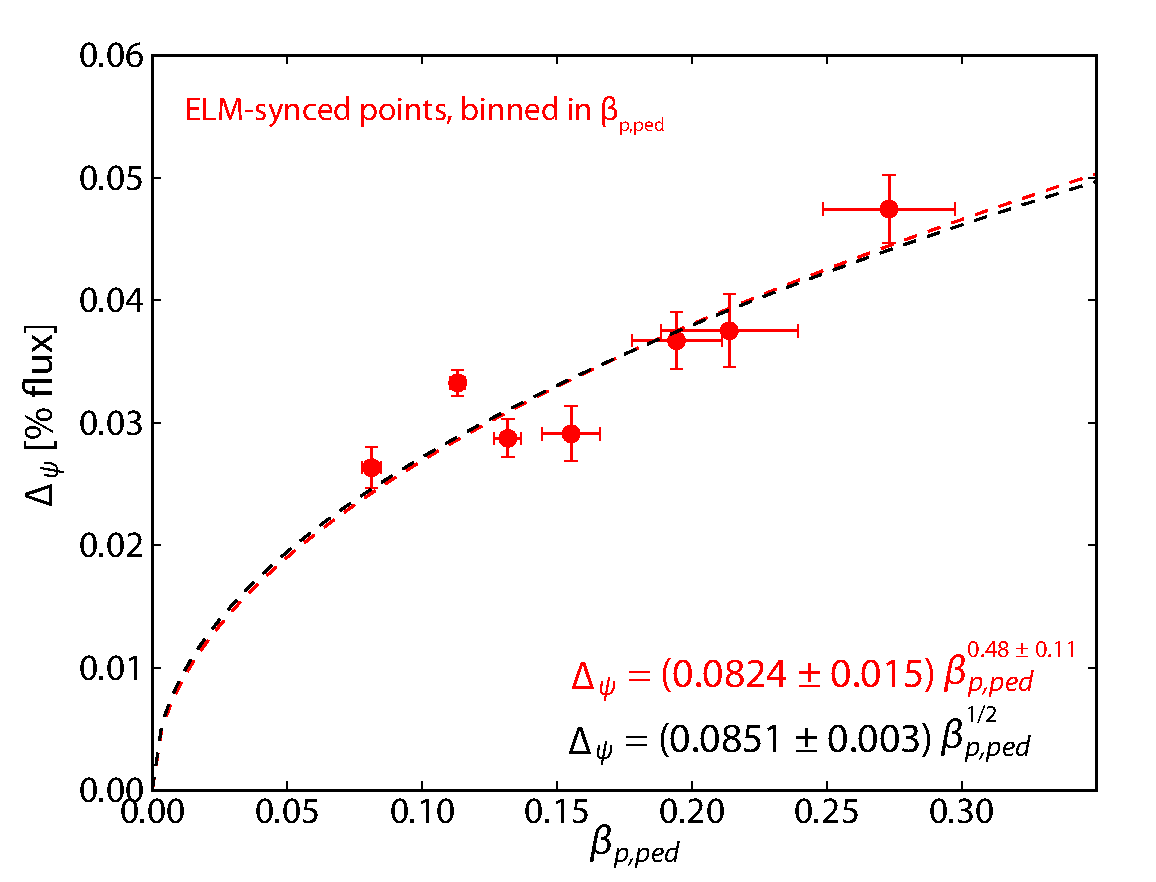
\includegraphics[width=100mm]{graphics/ELMy/betap_deltapsi_elmsync_betabin.pdf}}
\end{figure}

Prediction of the pedestal width is difficult, given the robust width of the pressure pedestal (typically 3-5\% of poloidal flux space, corresponding to $\sim \SI{5}{\milli\meter}$ on C-Mod).  The EPED model correctly recovers this robustness (within the expected $\pm 20\%$ prediction error), as shown in \cref{fig:elmy_deltapsi_eped}.  As seen in \cref{fig:elmy_betap_deltapsi_elmsync}, ELM-synchronized pedestals are typically somewhat wider than their ensemble-averaged counterparts, commensurate with the increased $\beta_{p,ped}$ at the maximum of the ELM cycle while the pedestal structure is limited throughout most of the ELM cycle by KBM turbulence\gnote{reword this}.  A comparison of the ELM-synced pedestal widths versus EPED1.63 prediction is shown in \cref{fig:elmy_deltapsi_elmsync}.\nicesectionending

\begin{figure}
 \pushtooutside
 \fcapside[60mm]{\caption[Measured ensemble-averaged pedestal width versus EPED predictions.]{Measured EPED pedestal width $\Delta_\psi = (\Delta_{n_e} + \Delta_{T_e})/2$ in ensemble-averaged pedestals versus EPED1.63-predicted pedestal widths.  Magnetic-field groups are indicated by color.  THe dashed line indicates perfect agreement with EPED prediction.  Pedestals widths are robust on C-Mod, restricted to $\sim 2-5\%$ of poloidal flux.  The EPED model reproduces this trait within expected prediction error.}\label{fig:elmy_deltapsi_eped}}{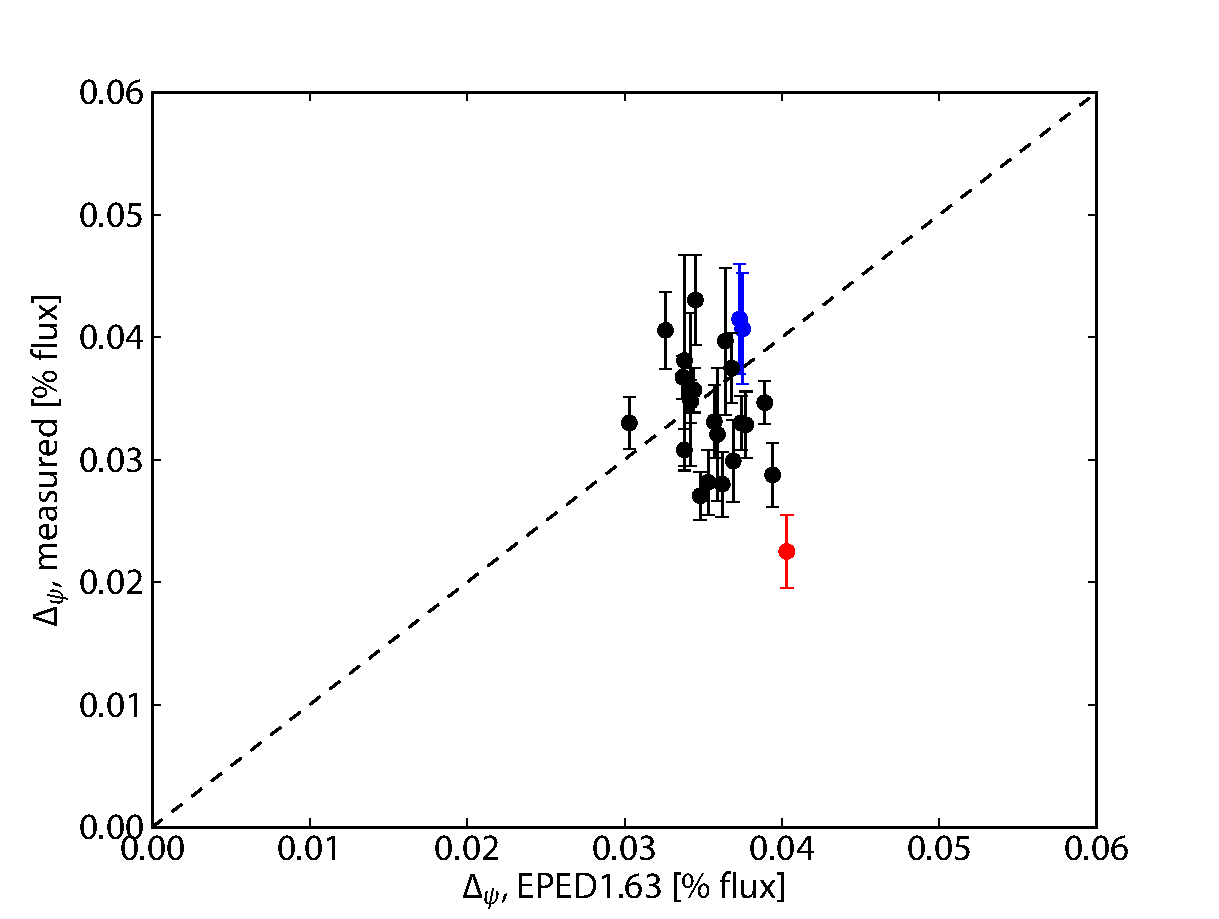
\includegraphics[width=100mm]{graphics/ELMy/deltapsi_EPED_meas.pdf}}
\end{figure}

\begin{figure}
 \pushtooutside
 \fcapside[60mm]{\caption[Measured ELM-synced pedestal width versus EPED predictions.]{Measured pedestal width $\Delta_\psi$ versus EPED1.63 predicted width.  Ensemble-averaged points are shown in black, while corresponding ELM-synchronized points are shown in red.  ELM-synced pedestals are typically somewhat wider, although still lie within the $\pm 20\%$ expected error for EPED.}\label{fig:elmy_deltapsi_elmsync}}{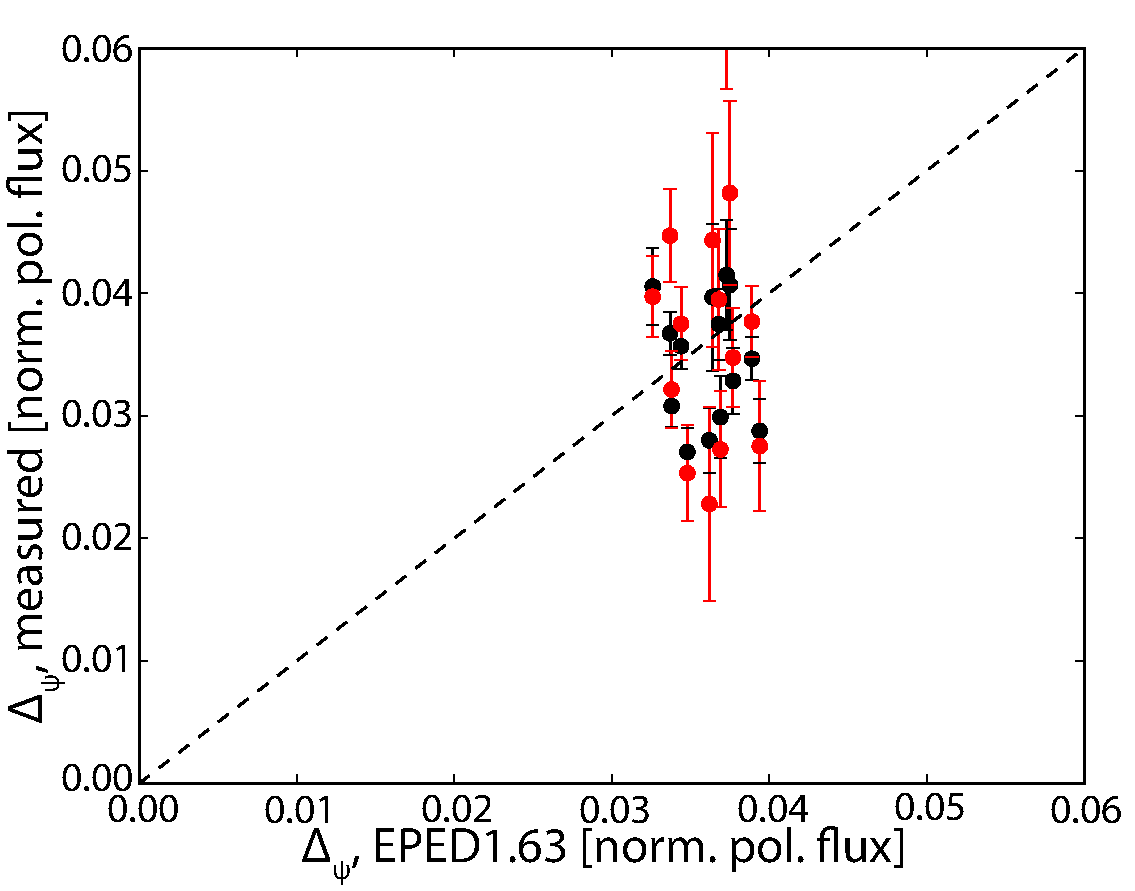
\includegraphics[width=100mm]{graphics/ELMy/deltapsi_EPED_elmsync.pdf}}
\end{figure}

\section{Engineering Parameter Scan}\label{sec:elmy_engineer}

The ELMy H-mode experiments presented here significantly expanded the parameter range available for the regime on Alcator C-Mod, including a broad scan in plasma current ($400-1100\;\si{\kilo\ampere}$) and toroidal magnetic field ($3.5, 5.4, 8.0\;\si{\tesla}$), as well as sweeps of elongation ($1.45 < \kappa < 1.55$) and collisionality ($0.25 < \nu_{95}^* < 6$).  This sweep entailed a factor of $\sim 7$ sweep in pedestal pressure -- notably, this expanded the range of pressure pedestals tested against the EPED model to within a factor of two of the target pedestal thermal pressure for ITER \cite{Snyder2011}.

\subsection{$I_p$ Scan}\label{subsec:elmy_ip}

\begin{figure}[p]
 \pushtooutside
 \ffigbox[\FBwidth]{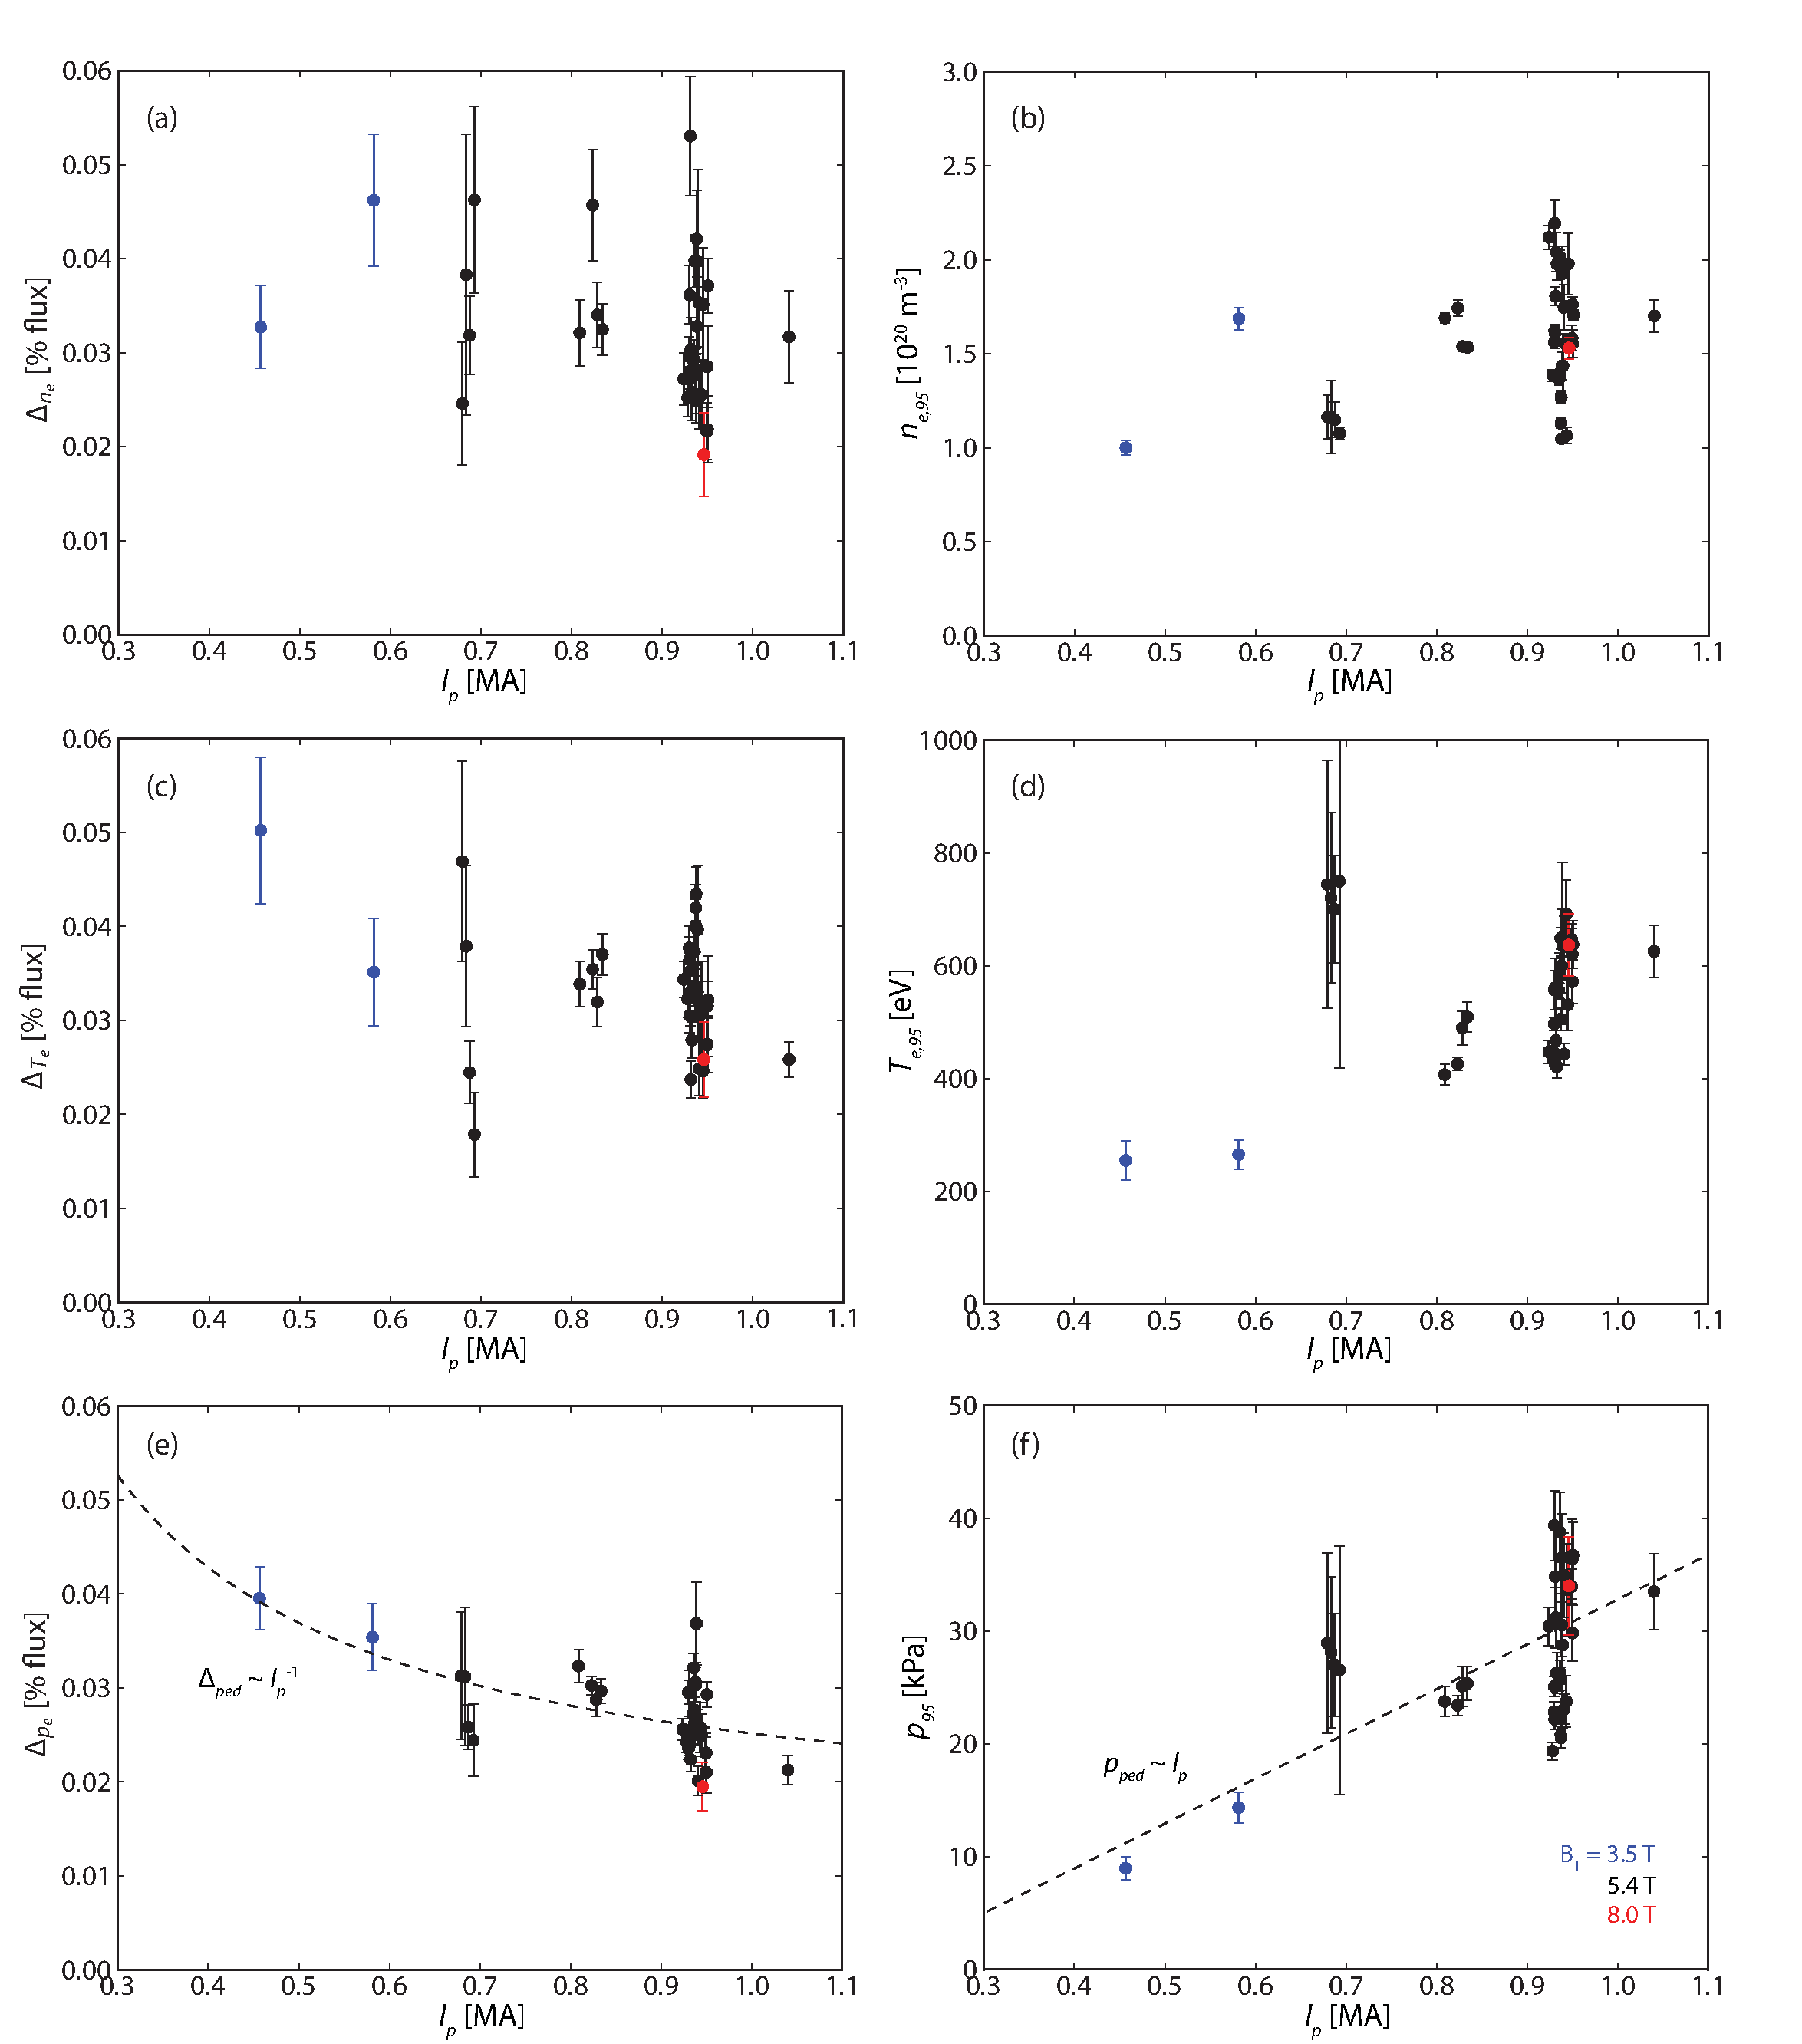
\includegraphics[width=150mm]{graphics/ELMy/Ip_scan.pdf}}{\caption[Plasma current scalings of the density, temperature, and pressure pedestals.]{Plasma current scalings of the density, temperature, and pressure pedestal widths and heights.  Magnetic-field sets are differentiated by color.  While the density and temperature pedestals independently show little systematic dependence of their widths on plasma current, the pressure pedestal width shows a exhibits a $\Delta_{ped} \sim I_p^{-1}$ trend.  The $n_e$ and $T_e$ pedestal heights both positively trend with current, although with significant scatter -- inverse trends between the two are consistent with the zero'th-order approximation of MHD-limited ELMy pedestals lying on a curve of fixed $\beta_{p,ped}$ for a given shaping/field configuration.  The pressure pedestal height shows a trend of $p_{ped} \sim I_p$, such that the pressure pedestal is consistent with the expected $\nabla p \sim I_p^2$ scaling.}\label{fig:elmy_ipscan}}
\end{figure}

Trends of the density, temperature, and pressure pedestal widths and heights with plasma current are shown in \cref{fig:elmy_ipscan}.  Previous experiments in EDA H-modes \cite{Hughes2007} demonstrated a robust linear dependence of the pedestal density on plasma current; a similar trend is found in ELMy H-mode (\cref{fig:elmy_ipscan}, (b)), albeit with a significantly less robust dependence.  A weak positive trend of the pedestal temperature (\cref{fig:elmy_ipscan}, (d)) is also seen, but is insufficient as a unique predictor.  The combined pressure pedestal ($p = 2 n_e T_e$) exhibits a $p_{95} \sim I_p$ trend, with some scatter.  

The density and temperature pedestal widths individually show no systematic dependence on the plasma current.  The compined pressure pedestal width -- although varying little over the range of 3-5\% of poloidal flux -- an inverse trend $\Delta_p \sim I_p^{-1}$ is discernable.  However, there is significant covariance between the plasma current and magnetic field, particularly at the low-$I_p$/low-$B_T$ points -- as some pedestal observations have asserted a broader pedestal at low field \cite{Hughes2002}\gnote{check this!}, this is a possible conflating factor.

These observations are generally consistent with historical observations of the ELMy H-mode pedestal -- the combined $p_{ped} \sim I_p$ and $\Delta_p \sim I_p^{-1}$ trends indicate a pressure gradient limit, $\nabla p \sim I_p^2$, consistent with pedestals limited by ballooning MHD instability, as described in \cref{sec:mod_pb}.  Moreover, the pressure pedestal width trend is consistent with the previously-observed constraint from kinetic-ballooning turbulence, $\Delta_p \sim \beta_{p,ped}^{1/2} \sim \sqrt{p_{ped}}/I_p$, with the scatter in $\Delta_p \sim I_p^{-1}$ due to pressure variation.  Previous experiments in H-mode\gnote{check refs} have observed a trend of $p_{ped} \sim I_p^2$ with no dependence of the pedestal width on current; however, this is consistent with the ballooning limit of $\nabla p \sim I_p^2$, and may be attributed to the small range over which the pedestal width varies on a given machine.  In the C-Mod cases as well, the pedestal width varies over a sufficiently small range that, to 
lowest order, the ballooning limit may be approximated as a limit on $\beta_{p}$ at the pedestal top.  This is shown in \cref{fig:elmy_neBp_TeBp} (see also \cref{fig:hcr_elmybetas}), showing the pedestal density versus temperature normalized to the poloidal field.  This normalization accounts for plasma-current differences between points, as well as rendering hyperbolae in the parameter space as contours of fixed $\beta_{p,ped}$.  At a given shaping, ELMy H-modes lie roughly on a contour of fixed $\beta_{p,ped}$, with stronger shaping allowing a higher attainable poloidal beta.

\begin{figure}[t]
 \pushtooutside
 \fcapside[60mm]{\caption[Pedestal density versus temperature normalized to poloidal field.]{Pedestal density vs. temperature normalized to poloidal field (accounting for variation in plasma current) such that hyperbolae in the parameter space are curves of fixed $\beta_{p,ped}$.  At a given shaping, ELMy H-mode pedestals are to lowest order constrained to fixed $\beta_{p,ped}$, with stronger shaping allowing greater attainable $\beta_p$.}\label{fig:elmy_neBp_TeBp}}{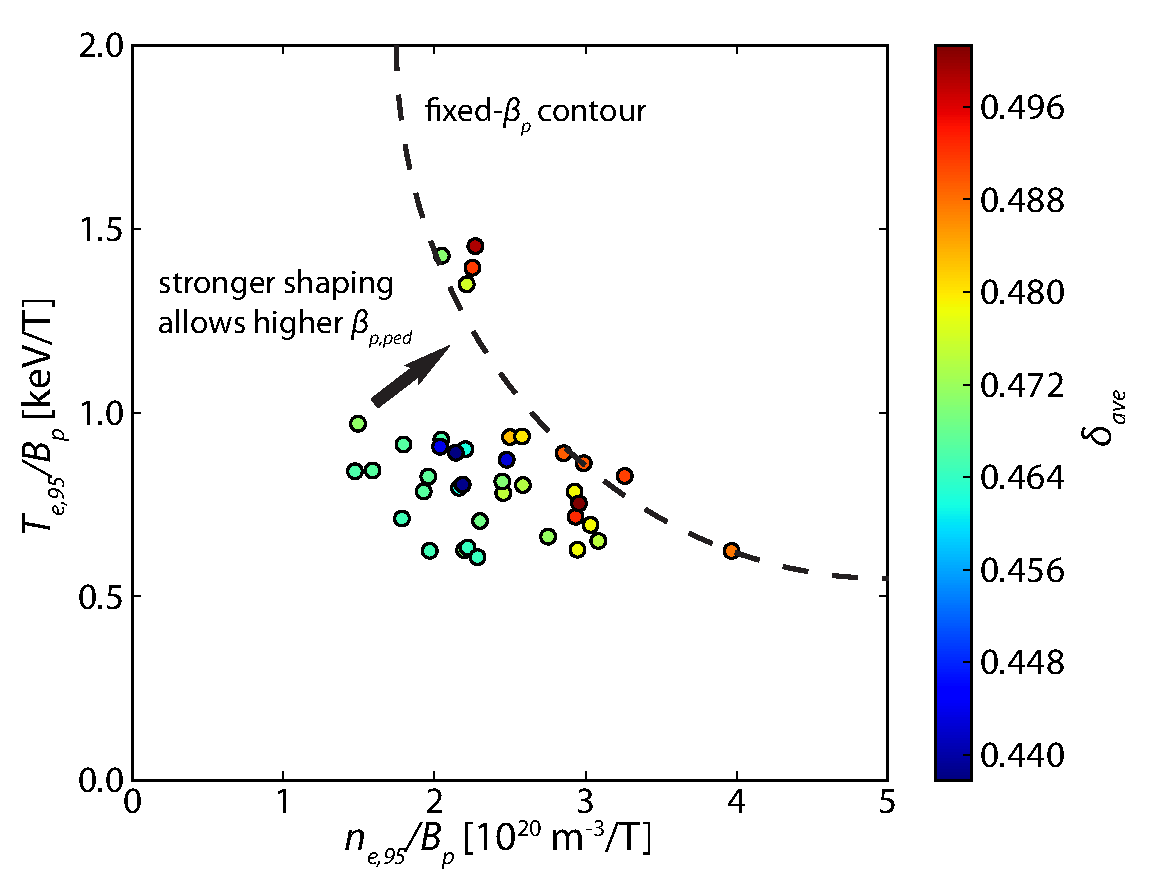
\includegraphics[width=100mm]{graphics/ELMy/neBp_TeBp_deltaave.pdf}}
\end{figure}

Pre-EPED models accounting for pressure-gradient limits assumed the pressure pedestal height would be governed simply by $p_{ped} \sim \nabla p \times \Delta_p$, with $\nabla p$ limited by MHD stability and a separate constraint for the pedestal width\gnote{better wording?}.  The ballooning limit was couched by Saibene \emph{et al.} \cite{Saibene1999} as $\nabla p \sim I_p^2 f_{sh}$, where $f_{sh}$ is a function describing the edge magnetic shear.  Taking the pedestal width to be governed by poloidal gyroradius $\rho_{i,pol} \sim \sqrt{T_e}/I_p$ (as was done by Saibene \emph{et al}.), this predicts $p_{ped} \sim I_p \sqrt{T_{e,ped}}$, as shown in \cref{fig:elmy_IprootTe_p95}.  However, the putative scaling of the pedestal width on $\rho_{i,pol}$ is readily conflated with the KBM-limited trend of pedestal width with $\beta_{p,ped}^{1/2} \sim \sqrt{n_e T_e}/I_p$.  Assuming a $\beta_{p,ped}$ limit on the pedestal width, we predict $p_{ped} \sim I_p \sqrt{n_{e,ped} T_{e,ped}}$, shown in \cref{fig:elmy_IprootneTe_p95} to be a significantly better predictor of the pedestal height.

%\begin{figure}[p]
 %\pushtooutside
 %\fcapside[60mm]{\caption[Pedestal pressure versus $I_p \sqrt{T_{e,95}}$]{Pedestal pressure versus $I_p \sqrt{T_{e,95}}$ -- effectively, the $p_{ped} \sim I_p^2 \rho_{i,pol}$ scaling predicted in \cite{Beurskens2011}.\note{check}}\label{fig:elmy_IprootTe_p95}}{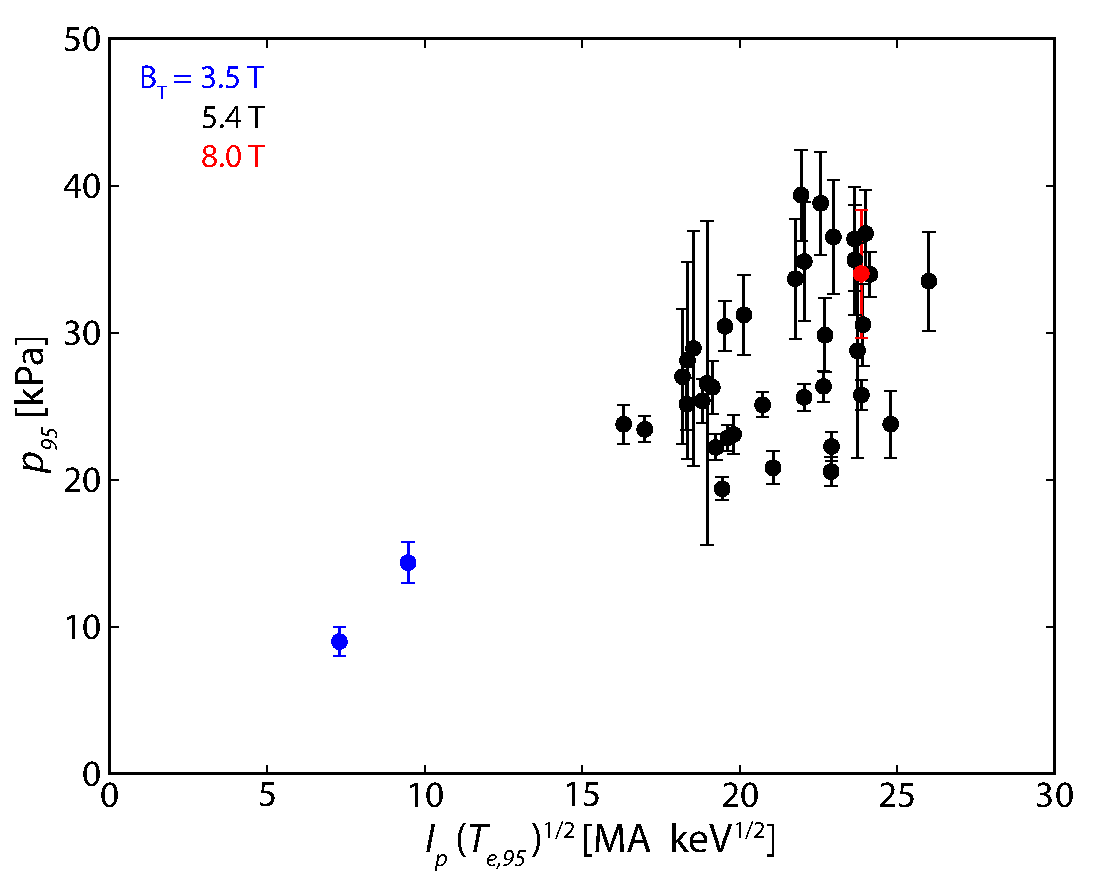
\includegraphics[width=100mm]{graphics/ELMy/IprootTe_p95.pdf}}
%\end{figure}
%
%\begin{figure}[p]
 %\pushtooutside
 %\fcapside[60mm]{\caption[Pedestal pressure versus $I_p \sqrt{n_{e,95} T_{e,95}}$]{Pedestal pressure versus $I_p \sqrt{n_{e,95} T_{e,95}}$ -- effectively, the $p_{ped} \sim I_p^2 \sqrt{\beta_{p,ped}}$ scaling predicted for a KBM-limited pedestal.}\label{fig:elmy_IprootneTe_p95}}{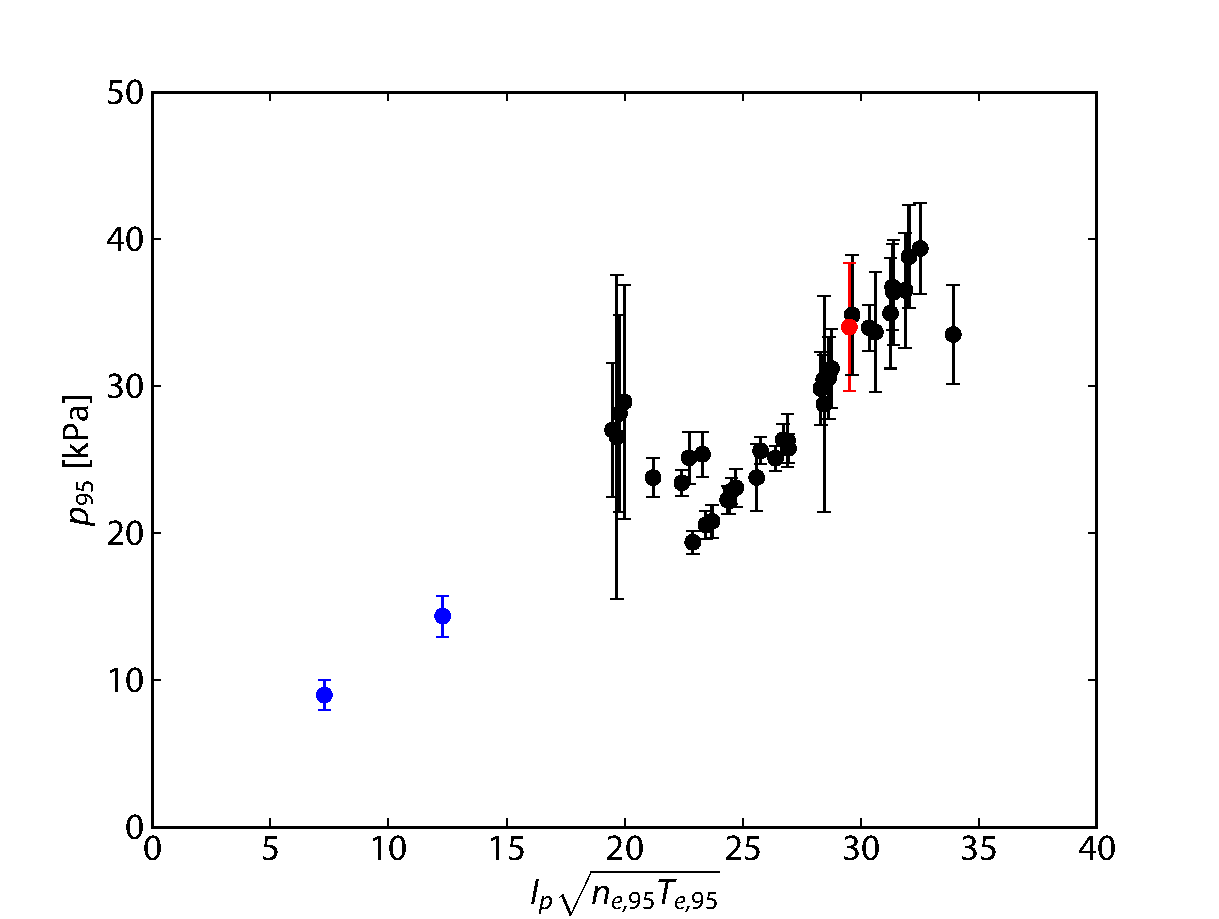
\includegraphics[width=100mm]{graphics/ELMy/IprootneTe_p95.pdf}}
%\end{figure}

\begin{figure}[ht]
 \pushtooutside
 \begin{floatrow}
  \ffigbox[\FBwidth]{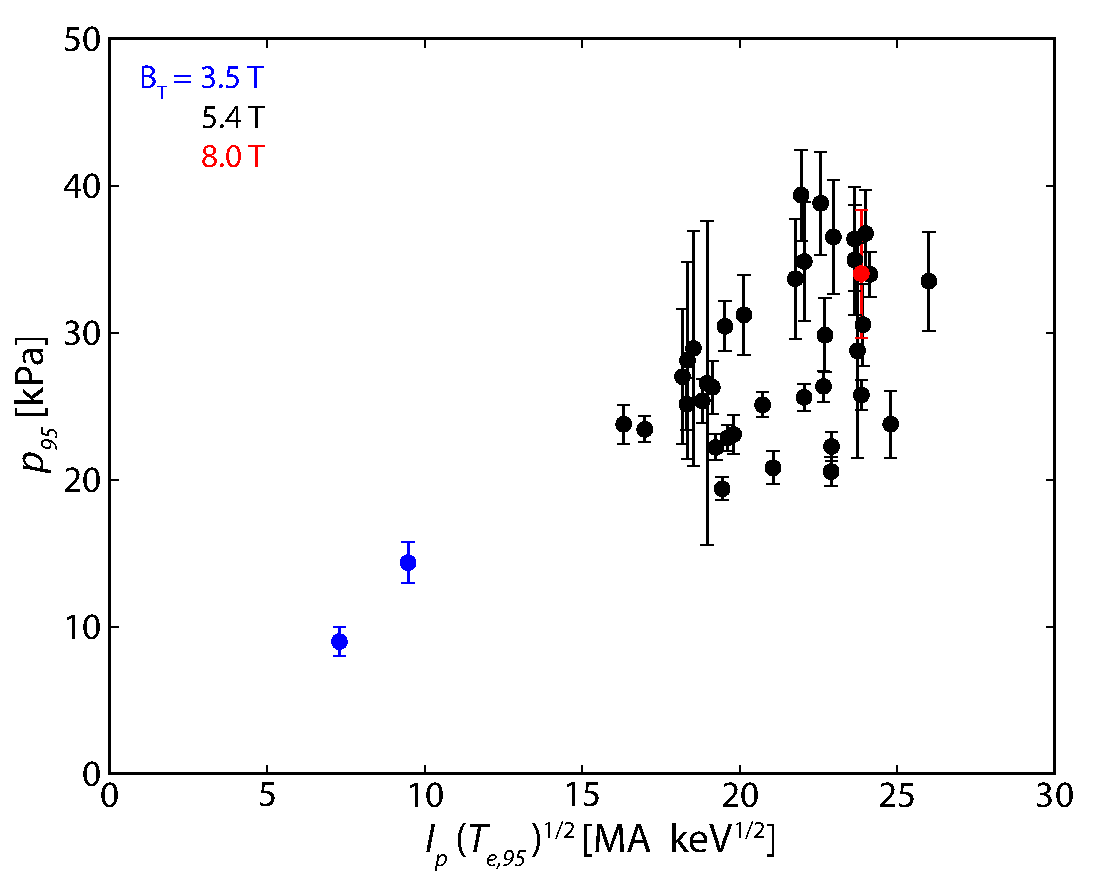
\includegraphics[width=75mm]{graphics/ELMy/IprootTe_p95.pdf}}{\caption[Pedestal pressure versus $I_p \sqrt{T_{e,95}}$]{Pedestal pressure versus $I_p \sqrt{T_{e,95}}$ -- effectively, the $p_{ped} \sim I_p^2 \rho_{i,pol}$ scaling predicted in \cite{Beurskens2011}.}\label{fig:elmy_IprootTe_p95}}
  \ffigbox[\FBwidth]{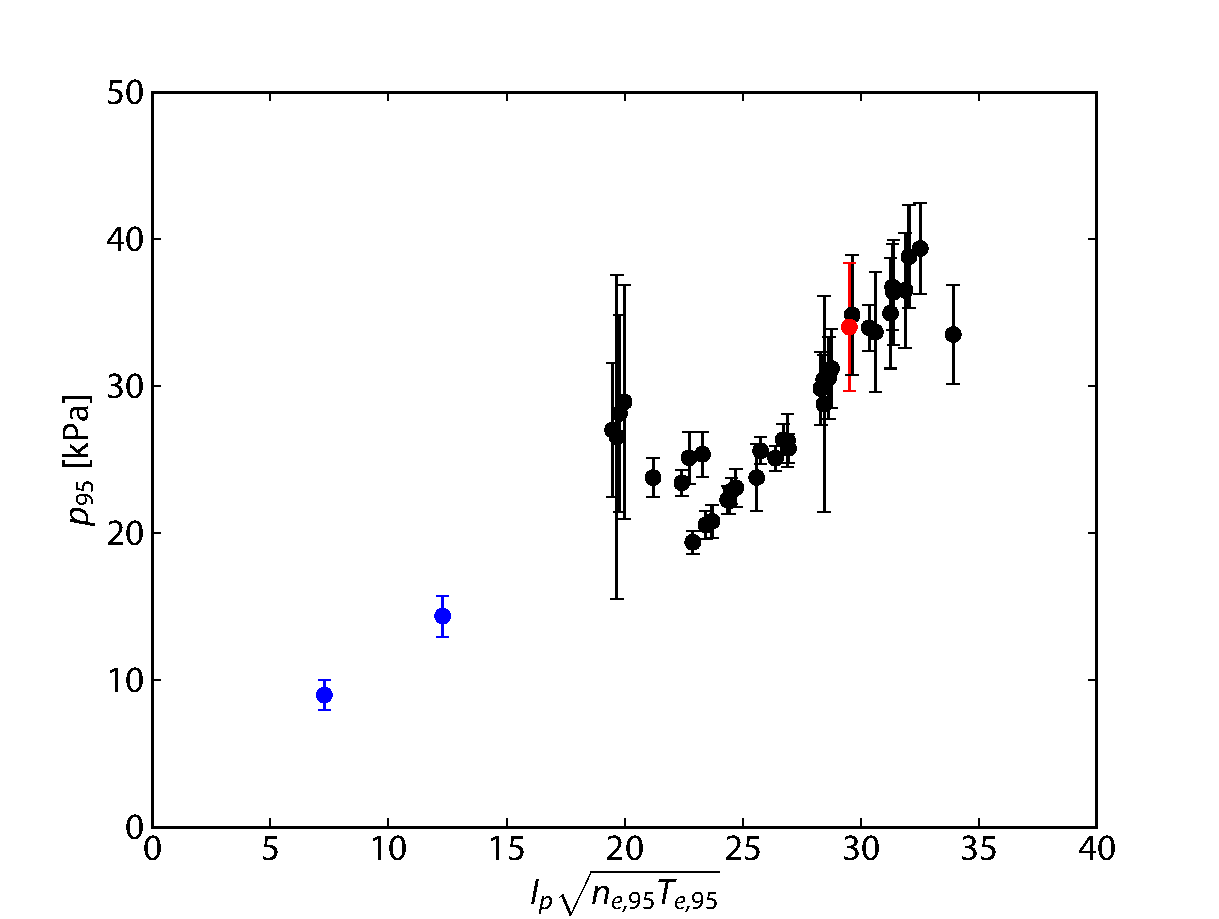
\includegraphics[width=75mm]{graphics/ELMy/IprootneTe_p95.pdf}}{\caption[Pedestal pressure versus $I_p \sqrt{n_{e,95} T_{e,95}}$]{Pedestal pressure versus $I_p \sqrt{n_{e,95} T_{e,95}}$ -- effectively, the $p_{ped} \sim I_p^2 \sqrt{\beta_{p,ped}}$ scaling predicted for a KBM-limited pedestal.}\label{fig:elmy_IprootneTe_p95}}
 \end{floatrow}
\end{figure}

% \subsection{Power Scan}\label{subsec:elmy_power}
% 
% \begin{figure}[ht]
%  \pushtooutside
%  \fcapside[60mm]{\caption[Pedestal $T_e$ versus net heating power normalized to density.]{Pedestal temperature versus net heating power ($P_{net} = P_{ICRF} + P_{Ohm} - P_{rad} - dW/dt$) normalized to pedestal density (a surrogate for heat flux through the pedestal).  At a given value of plasma current (shown by the colorbar), there is little variation of the pedestal temperature with $P_{net}/n_{e,95}$.  Rather, heating power modulates the ELM frequency, increasing heat transport.}\label{fig:elmy_Pneped_Tped}}{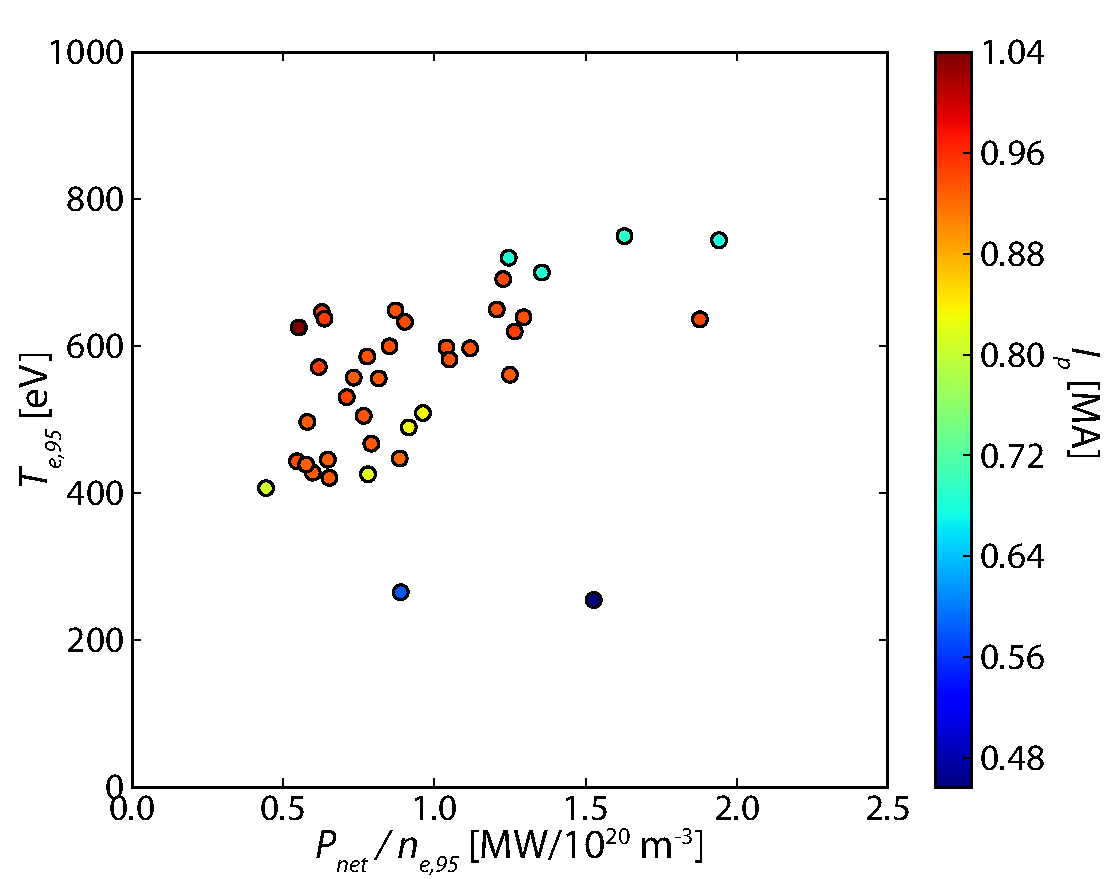
\includegraphics[width=100mm]{graphics/ELMy/Pne95_Te95_Ip.pdf}}
% \end{figure}
% 
% \begin{figure}[ht]
%  \pushtooutside
%  \fcapside[60mm]{\caption[Pedestal pressure versus net heating power.]{Pedestal pressure versus net heating power $P_{net} = P_{ICRF} + P_{Ohm} - P_{rad} - dW/dt$).  At a given value of the plasma current (shown by the colorbar), there is little variation of pedestal pressure with $P_{net}$.  Rather, heating power modulates the ELM frequency ($f_{ELM} \sim P_{heat}$ for type-I ELMs \note{cite}), increasing outward energy transport to maintain the pressure pedestal on a line of fixed $\beta_{p,ped}$ for a given shape.}\label{fig:elmy_Pnet_pped}}{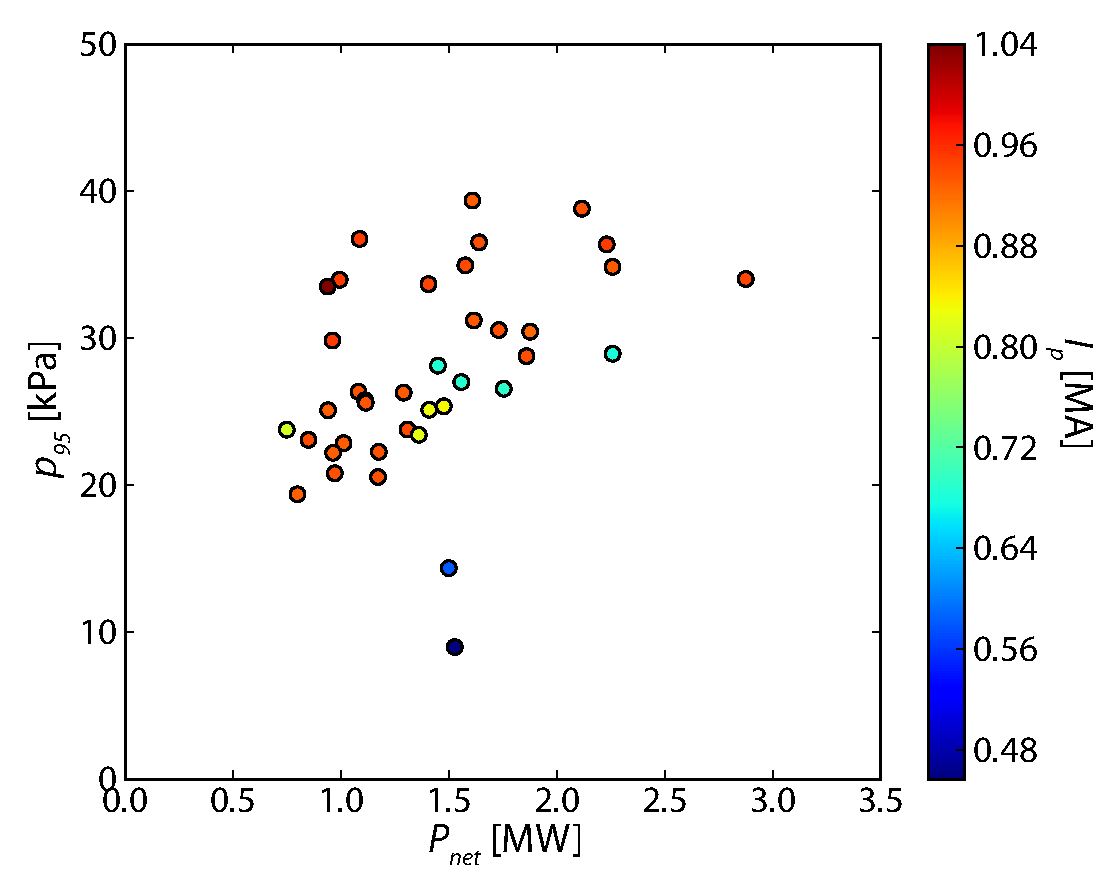
\includegraphics[width=100mm]{graphics/ELMy/Pnet_p95_Ip.pdf}}
% \end{figure}
% 
% The response of the pedestal to heating power is consistent with previous observations in MHD-limited pedestals\gnote{cites, elaboration?}.  Examined against net heating power $P_{net} = P_{ICRF} + P_{Ohm} - P_{rad} - dW/dt$ normalized to the pedestal density (effectively, heat flux through the pedestal), the temperature pedestal height (shown in \cref{fig:elmy_Pneped_Tped}) shows little response within a given target plasma current.  \note{arguments based on profile stiffness...}
% 
% Similarly, the pressure pedestal shows a weak response to net heating power (\cref{fig:elmy_Pnet_pped}), with the attainable pressure instead predominantly set by current (see \cref{subsec:elmy_ip}) and shaping (due to the stabilizing effects of strong shaping on peeling-ballooning MHD -- see \cref{fig:elmy_neBp_TeBp} for the influence of shaping on attainable $\beta_{p,ped}$).  Previous observations in ELMy H-mode\gnote{cites or ref lit review} observed a dependence of the ELM repetition frequency with heating power in type-I ELMs, such that for relatively fixed energy loss per ELM (typically 2-6\% of pedestal stored energy\gnote{check}) increased heating power increases the average ELM power loss ($\langle P_{ELM} \rangle \sim f_{ELM} \cdot \delta W_{ELM}$) to maintain $P_{ELM}$ at a fixed fraction of total heating power.  This increased heat transport due to ELM instabilities is reflected in the ITER98 scaling (\cref{eq:tau98}), $\tau_E \sim P_{net}^{-0.69}$.  As the total stored energy scales linearly 
% with the pedestal pressure \cite{Kinsey2011}, $W \sim p_{ped}$, and in a stationary plasma ($dW/dt \approx 0$) $W \sim P_{net} \tau_E$, we 
% expect $p_{ped} \sim P_{net}^{0.3}$ based on global scalings alone.\nicesectionending

\section{Pedestal Width Response}\label{sec:elmy_width}

\subsection{Alternate Width Models}\label{subsec:elmy_width_oldmodels}

\begin{figure}
 \pushtooutside
 \fcapside[60mm]{\caption[$\Delta_{n_e}$ versus $n_{e,ped}$]{Density pedestal width versus pedestal density.  Contrary to expectations from neutral-penetration models (see \cref{subsec:mod_neutral}), there is little systematic variation of the density pedestal width and height.}\label{fig:elmy_ne_deltan}}{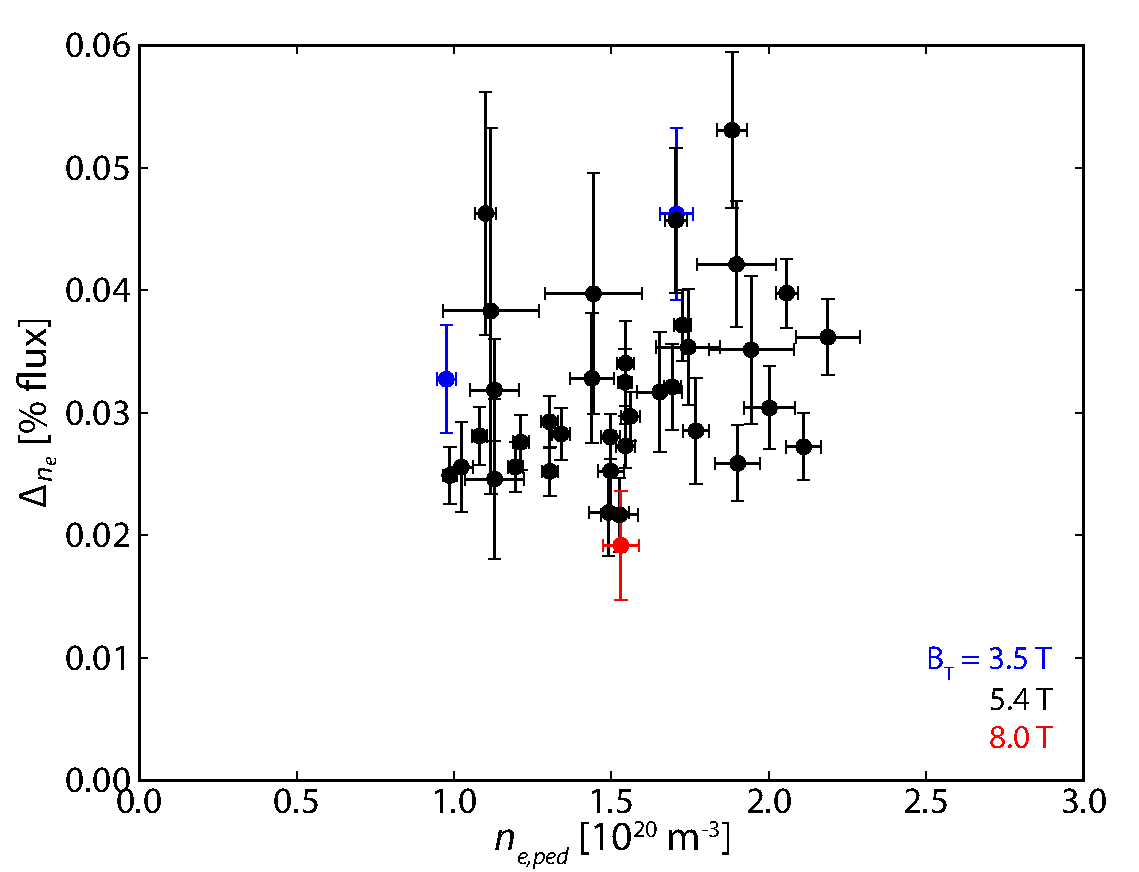
\includegraphics[width=100mm]{graphics/ELMy/neped_deltan.pdf}}
\end{figure}

\begin{figure}
 \pushtooutside
 \ffigbox[\FBwidth]{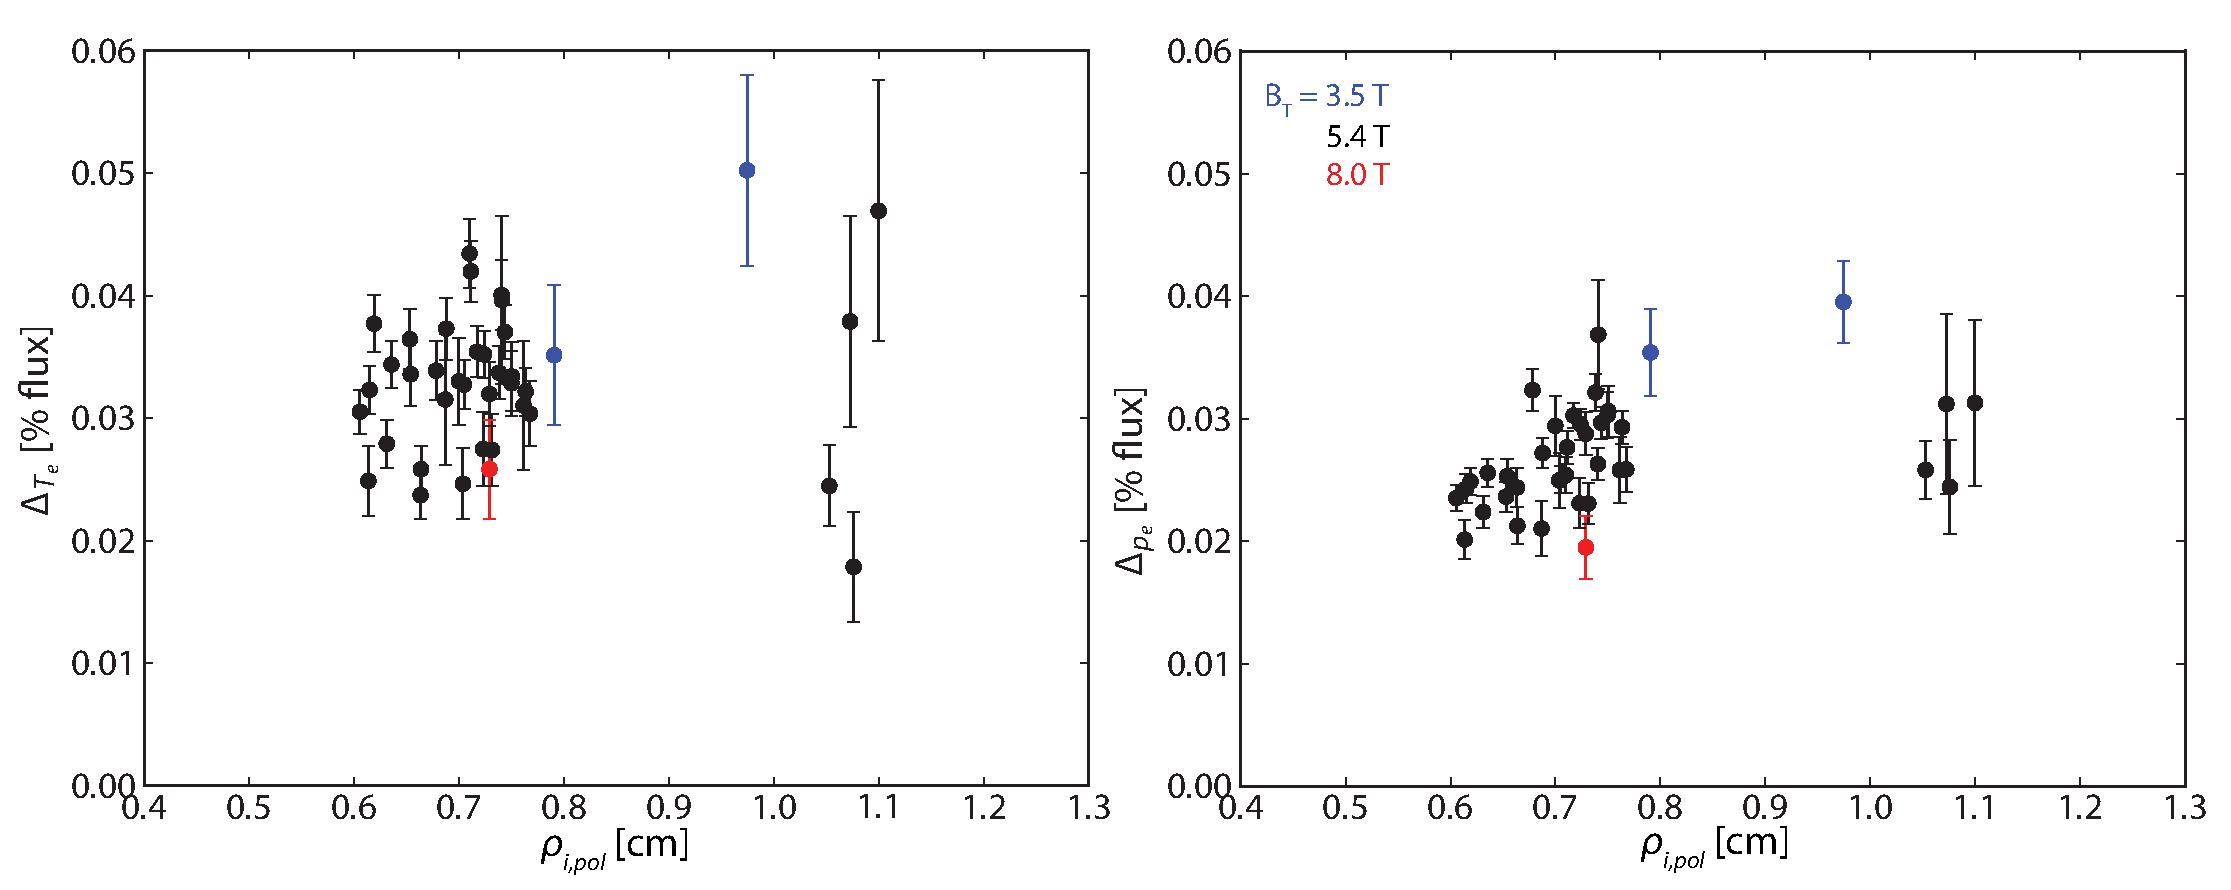
\includegraphics[width=150mm]{graphics/ELMy/rhoipol_deltas.pdf}}{\caption[$\Delta_{T_e}$ and $\Delta_{p}$ versus $\rho_{i,pol}$]{Temperature and pressure pedestal widths versus poloidal gyroradius.  The temperature pedestal width shows no systematic variation with $\rho_{i,pol}$.  A weak trend is possible in the pressure pedestal width, comparable to the the trend of $\Delta_p \sim \beta_{p,ped}^{1/2}$ (due to the strong covariance between $\rho_{i,pol}$ and $\beta_{p,ped}$).  However, this trend is overruled in favor of a poloidal beta scaling by other observations.}\label{fig:elmy_rhoipol_deltas}}
\end{figure}

Initial models for the pedestal width (see \cref{sec:mod_early}) led to several easily-testable predictions -- first, neutral-penetration models (\cref{subsec:mod_neutral}) predict a scaling of the density pedestal $\Delta_{n_e} \sim 1/n_{e,ped}$, while transport-driven models predict temperature/pressure pedestal widths limited by poloidal gyroradius, or equivalently the banana orbit width (\cref{subsec:mod_ionorbitloss}).  The density pedestal width is shown against pedestal density in \cref{fig:elmy_ne_deltan} -- while there is high scatter in the data, with both the pedestal density and measured width $\Delta_{n_e}$ spanning more than a factor of two in variation, the densest region in the dataset shows a weak positive trend between density pedestal width and height.  This is directly contrary to the predictions from simple neutral-penetration models; however, it is consistent with previous observations in EDA H-mode \cite{Hughes2002}.  The measured temperature and pressure widths $\Delta_{T_e}$ and $\Delta_{p_e}$ are shown against $\rho_{i,pol}$ (the ion gyroradius evaluated with the poloidal field) in \cref{fig:elmy_rhoipol_deltas}.  In the case of the temperature pedestal width, no systematic variation with $\rho_{i,pol}$ is seen.  A possible weak trend for the pressure pedestal width is seen, with comparable spread to that seen in the pressure pedestal width versus $\beta_{p,ped}$.  However, as there is significant covariance between $\rho_{i,pol} \sim \sqrt{T_e}/I_p$ and $\beta_{p,ped} \sim \sqrt{n_e T_e}/I_p$, and the width scaling with $\beta_{p,ped}$ is seen to be a superior predictor (see \cref{fig:elmy_IprootneTe_p95}) this model should be discarded in favor of the $\Delta \sim \beta_{p,ped}^{1/2}$ scaling from KBM physics.  This is consistent with results from experiments designed to distinguish between $\rho_{i,pol}$ and $\beta_{p,ped}$ dependencies via isotope variation to exploit the mass dependence in $\rho_{i,pol}$ \cite{Urano2008} or pumping experiments to independently vary pedestal density and temperature at fixed pressure \cite{Osborne1998,Maggi2010}.

\subsection{Normalized Pedestal Width}\label{subsec:elmy_normwidth}

As detailed in \cref{subsec:elmy_eped_width}\gnote{ref to ch. 3 section?}, the scale factor in the dominant width scaling in ELMy H-mode, $\Delta \sim \beta_{p,ped}^{1/2}$, is most properly a weakly varying function of plasma shaping, collisionality, and other dimensionless parameters: $\Delta_\psi = G(\nu^*,\varepsilon,...) \beta_{p,ped}^{1/2}$ \cite{Snyder2011}.  These secondary dependencies in $G$ may be examined by normalizing the pedestal width (here we use the EPED width, $\Delta_\psi$, from \cref{eq:wid_eped}) to the fitted scaling $\Delta_\psi = 0.0857 \beta_{p,ped}^{1/2}$ (see \cref{fig:elmy_betap_deltapsi_all}).  

Normalized pedestal widths are shown against the range in toroidal fields in \cref{fig:elmy_Bt_deltanorm}.  The high scatter in the normalized pedestal widths at standard field ($\SI{5.4}{\tesla}$), along with the difficulty in attaining usable ELMy H-modes at low and high field, renders it difficult to conclusively establish a secondary scaling of the pedestal width with toroidal field.  While the comparatively broader pedestal at low field is consistent with some previous observations\gnote{cite Hughes... DIII-D observations too?}, the covariance between $B_T$ and $I_p$ (and therefore $\beta_p$) in the low-field phase of the experiment complicates this observation.

\begin{figure}
 \pushtooutside
 \fcapside[60mm]{\caption[Scaling of the normalized pedestal width with applied toroidal field.]{Scalings of the pedestal width $\Delta_\psi$, normalized to the dominant scaling $\Delta_\psi = 0.0857 \beta_{p,ped}^{1/2}$, with the applied toroidal field $B_T$.  Although the high scatter at standard $B_T$ and the sparsity of data at low and high field makes a conclusive scaling difficult, there is some indication of an inverse relation of pedestal width with toroidal field.}\label{fig:elmy_Bt_deltanorm}}{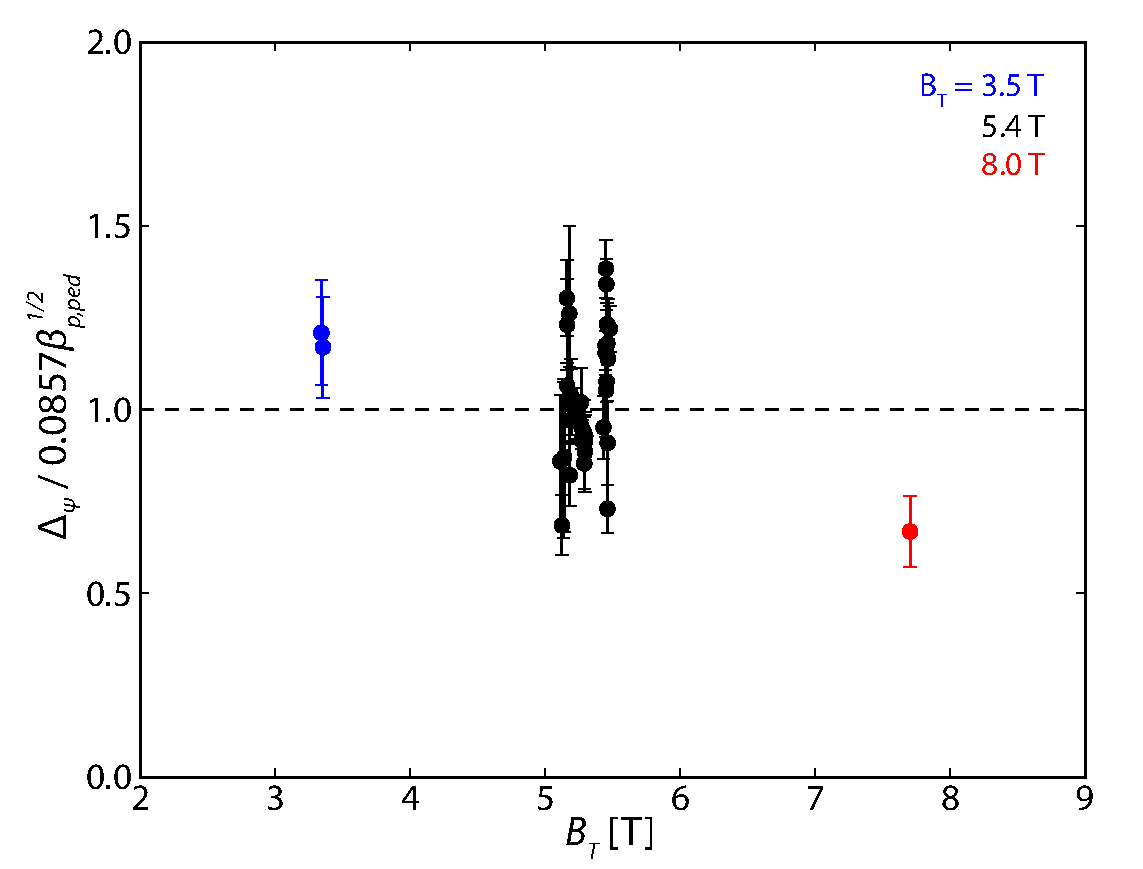
\includegraphics[width=100mm]{graphics/ELMy/Bt_deltanorm.pdf}}
\end{figure}

Similarly, normalized pedestal widths are shown against the plasma shaping parameters -- upper and lower triangularity $\delta_u$, $\delta_l$, average triangularity $\delta_{ave} = (\delta_l + \delta_u)/2$, and elongation $\kappa$ -- in \cref{fig:elmy_shaping_deltanorm}.  No clear secondary dependence of the normalized pedestal width (that is, in the scale function $G(\nu^*,\varepsilon,...)$) is seen in shaping: $\delta_l$, $\delta_{ave}$, and $\kappa$ exhibit no trend, while $\delta_u$ is unclear with the broadest widths (compared to the $\sim 0.0857 \beta_{p,ped}^{1/2}$ fit) at both the low and high extremes of the range in $\delta_u$.  Rather, the shaping dependence manifests as increased poloidal beta, and secondarily pedestal width, at stronger shaping -- increased shaping is known to have a stabilizing effect on ballooning MHD modes, increasing the normalized pressure gradient $\alpha_{MHD}$ at which the instability is triggered.  However, as the shaping range available for ELMy H-modes on C-Mod is restricted, weak dependences on shaping are still possible.

\begin{figure}
 \pushtooutside
 \ffigbox[\FBwidth]{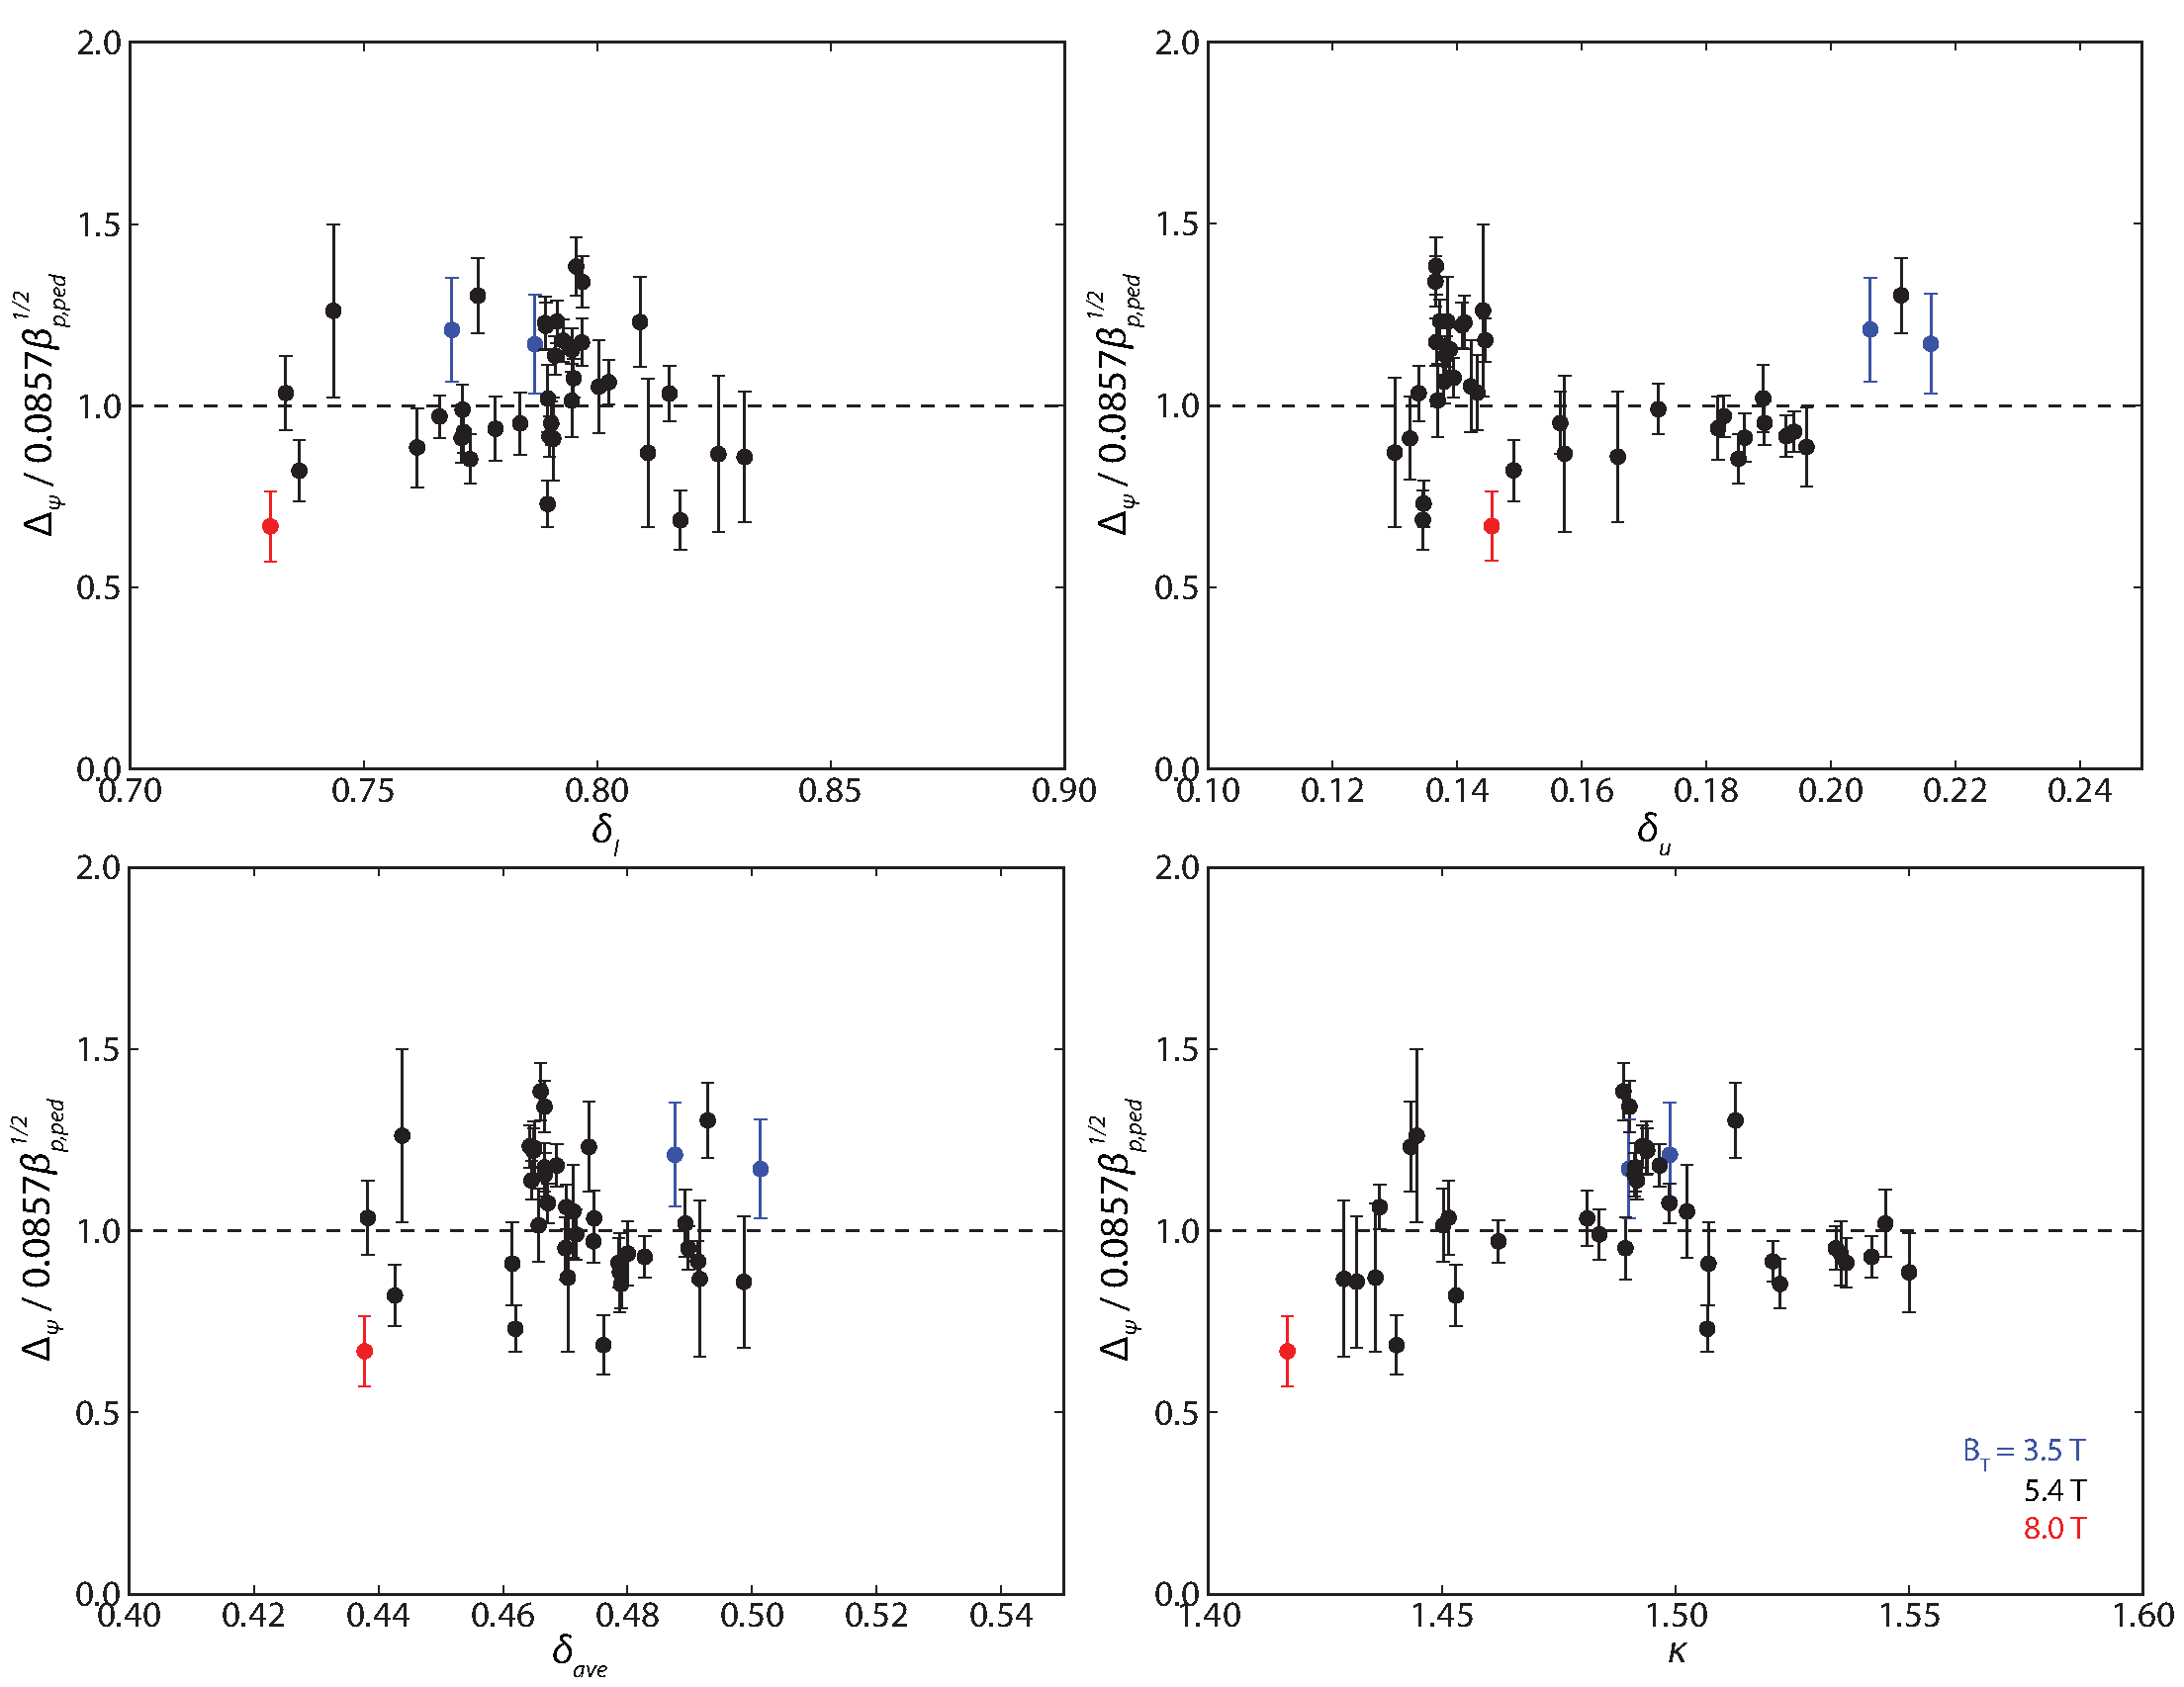
\includegraphics[width=150mm]{graphics/ELMy/shaping_deltanorm.pdf}}{\caption[Scalings of normalized pedestal width with shaping parameters.]{Scalings of the pedestal width $\Delta_\psi$ normalized to the dominant scaling $\Delta_\psi = 0.0857 \beta_{p,ped}^{1/2}$, with plasma shaping: upper, lower, and average triangularity ($\delta_l$, $\delta_u$, $\delta_{ave} = (\delta_u + \delta_l)/2$), and elongation $\kappa$.  No strong trend with shaping parameters is seen -- rather, the influence of plasma shaping is exhibited by increased $\beta_{p,ped}$ and pedestal width due to increased stability to peeling-ballooning MHD.}\label{fig:elmy_shaping_deltanorm}}
\end{figure}

Pedestal collisionality $\nu^*_{95}$ is anticipated as a controlling term in the scale function $G$, due both to its role in controlling ionization rate and neutral penetration, and its influence on bootstrap current density and the accompanying MHD effects in the pedestal.\gnote{cite, elaborate?}  However, across a broad range on collisionality, $0.25 < \nu^*_{95} < 6$, no systematic variation in the normalized pedestal width is seen (see \cref{fig:elmy_nustar_deltanorm}).  The highest collisionality points were obtained in cold, low-field discharges, possibly conflating the elevated pedestal width (relative to the $\sim 0.0857 \beta_{p,ped}^{1/2}$ fit) with possible broadening at reduced $B_T$.

While a primary dependence of the pedestal width on the gyroradius is ruled out (see the discussion in \cref{subsec:elmy_width_oldmodels} and \cref{fig:elmy_IprootneTe_p95}), a secondary gyroradius dependence in addition to the $\beta_{p}$ scaling is still possible -- for example, $\Delta_{ped} \sim \rho_{i,pol}^{0.2} \beta_{p,ped}^{0.5}$ found by Urano \emph{et al.} \cite{Urano2008}.  However, when the scale function $G$ is examined via trends of the normalized pedestal width versus normalized gyroradius $\rho^*_{95}$, shown in \cref{fig:elmy_rhostar_deltanorm}, no systematic dependence is seen.  Notably, the strong outlier for $\rho^*$ -- the high-$B_T$ case, shown to have a narrow pedestal compared to the expected scaling -- is nevertheless within the range of normalized width for the bulk of the dataset.  As such, no distinct dependence of the normalized width (equivalently, $G(\nu^*,\varepsilon,...)$) can be discerned from the data.\nicesectionending

\begin{figure}
 \pushtooutside
 \fcapside[60mm]{\caption[Scaling of normalized pedestal width with pedestal collisionality.]{Scaling of the normalized pedestal width $\Delta_\psi / 0.0857 \beta_{p,ped}^{1/2}$ versus pedestal collisionality $\nu^*_{95}$.  Low, standard, and high-field sets are indicated in blue, black, and red respectively.  No systematic variation is observed.}\label{fig:elmy_nustar_deltanorm}}{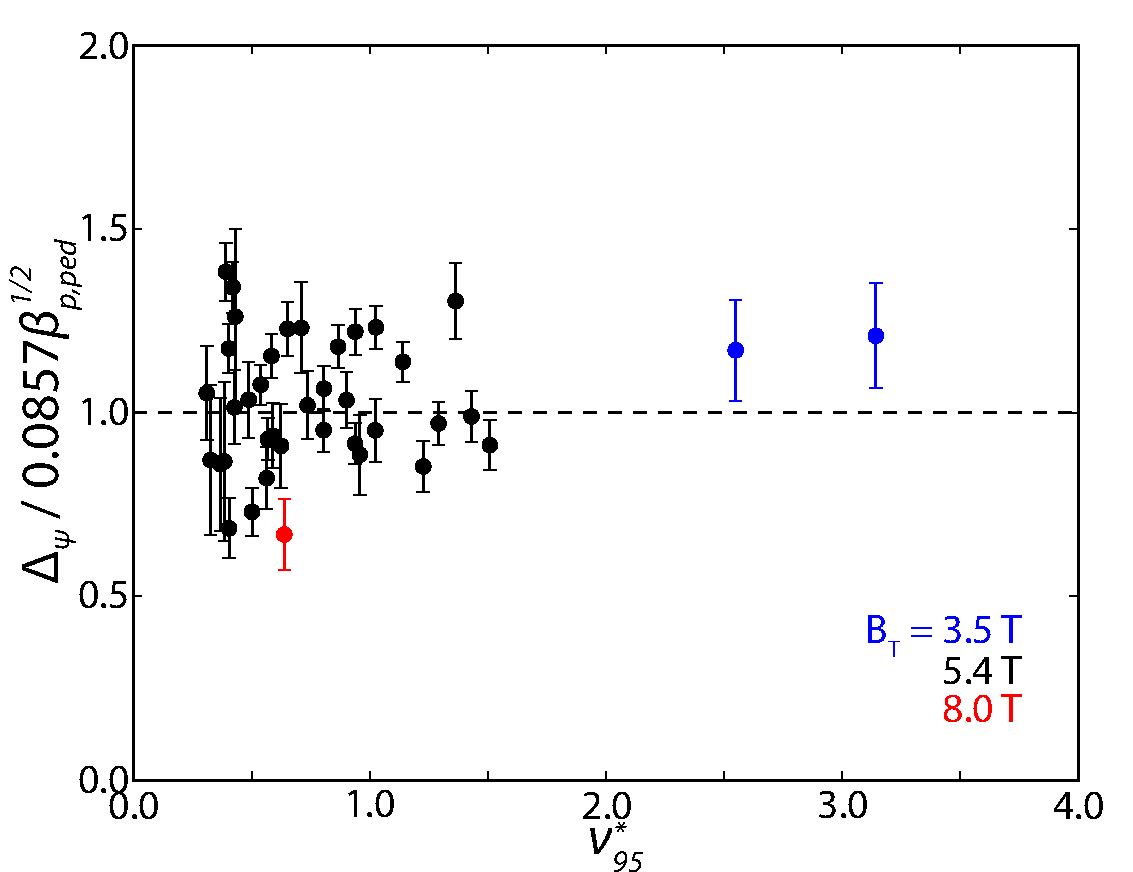
\includegraphics[width=100mm]{graphics/ELMy/nustar_deltanorm.pdf}}
\end{figure}

\begin{figure}
 \pushtooutside
 \fcapside[60mm]{\caption[Scaling of normalized pedestal width with normalized pedestal ion gyroradius.]{Scaling of the normalized pedestal width $\Delta_\psi / 0.0857 \beta_{p,ped}^{1/2}$ with normalized pedestal gyroradius $\rho^*_{95}$.  Low, standard, and high-field sets are indicated in blue, black, and red respectively.  No systematic variation is seen.}\label{fig:elmy_rhostar_deltanorm}}{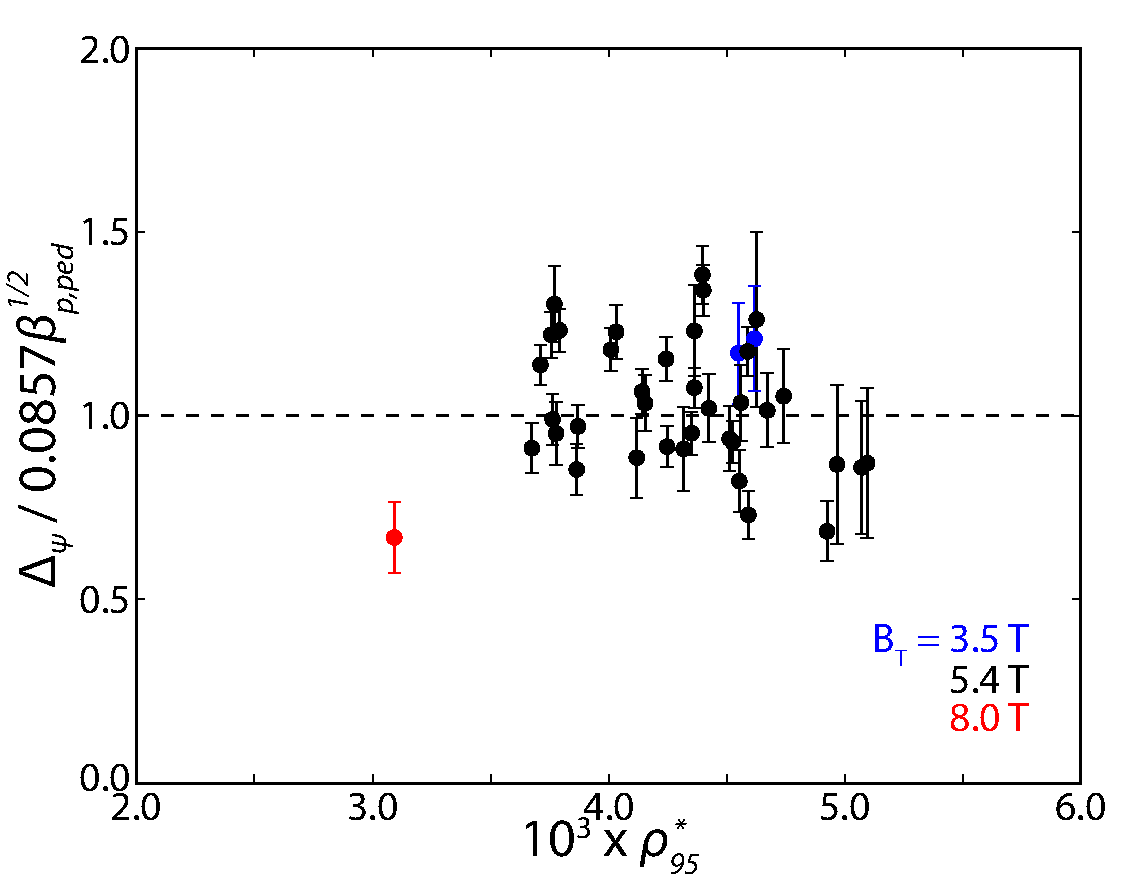
\includegraphics[width=100mm]{graphics/ELMy/rhostar_deltanorm.pdf}}
\end{figure}

\section{Conclusions}\label{sec:elmy_conclusion}



\nicechapterending

\bibliographystyle{../plainurl}
\bibliography{../references}